\chapter{Construction}

\section{Contruction}

The hodoscope was constructed in a purpose built environment in a re-purposed laboratory at The University of Edinburgh. The space was designed to minimize dust levels, exposure to UV light and provide a temperature controlled environment. The tent was constructed to isolate the detector elements for construction and fitted with an air filtration system, and specialist UV lighting that blocked out wavelengths shorter than the red part of the visible spectrum.

\begin{figure}[!ht]
	\centering
	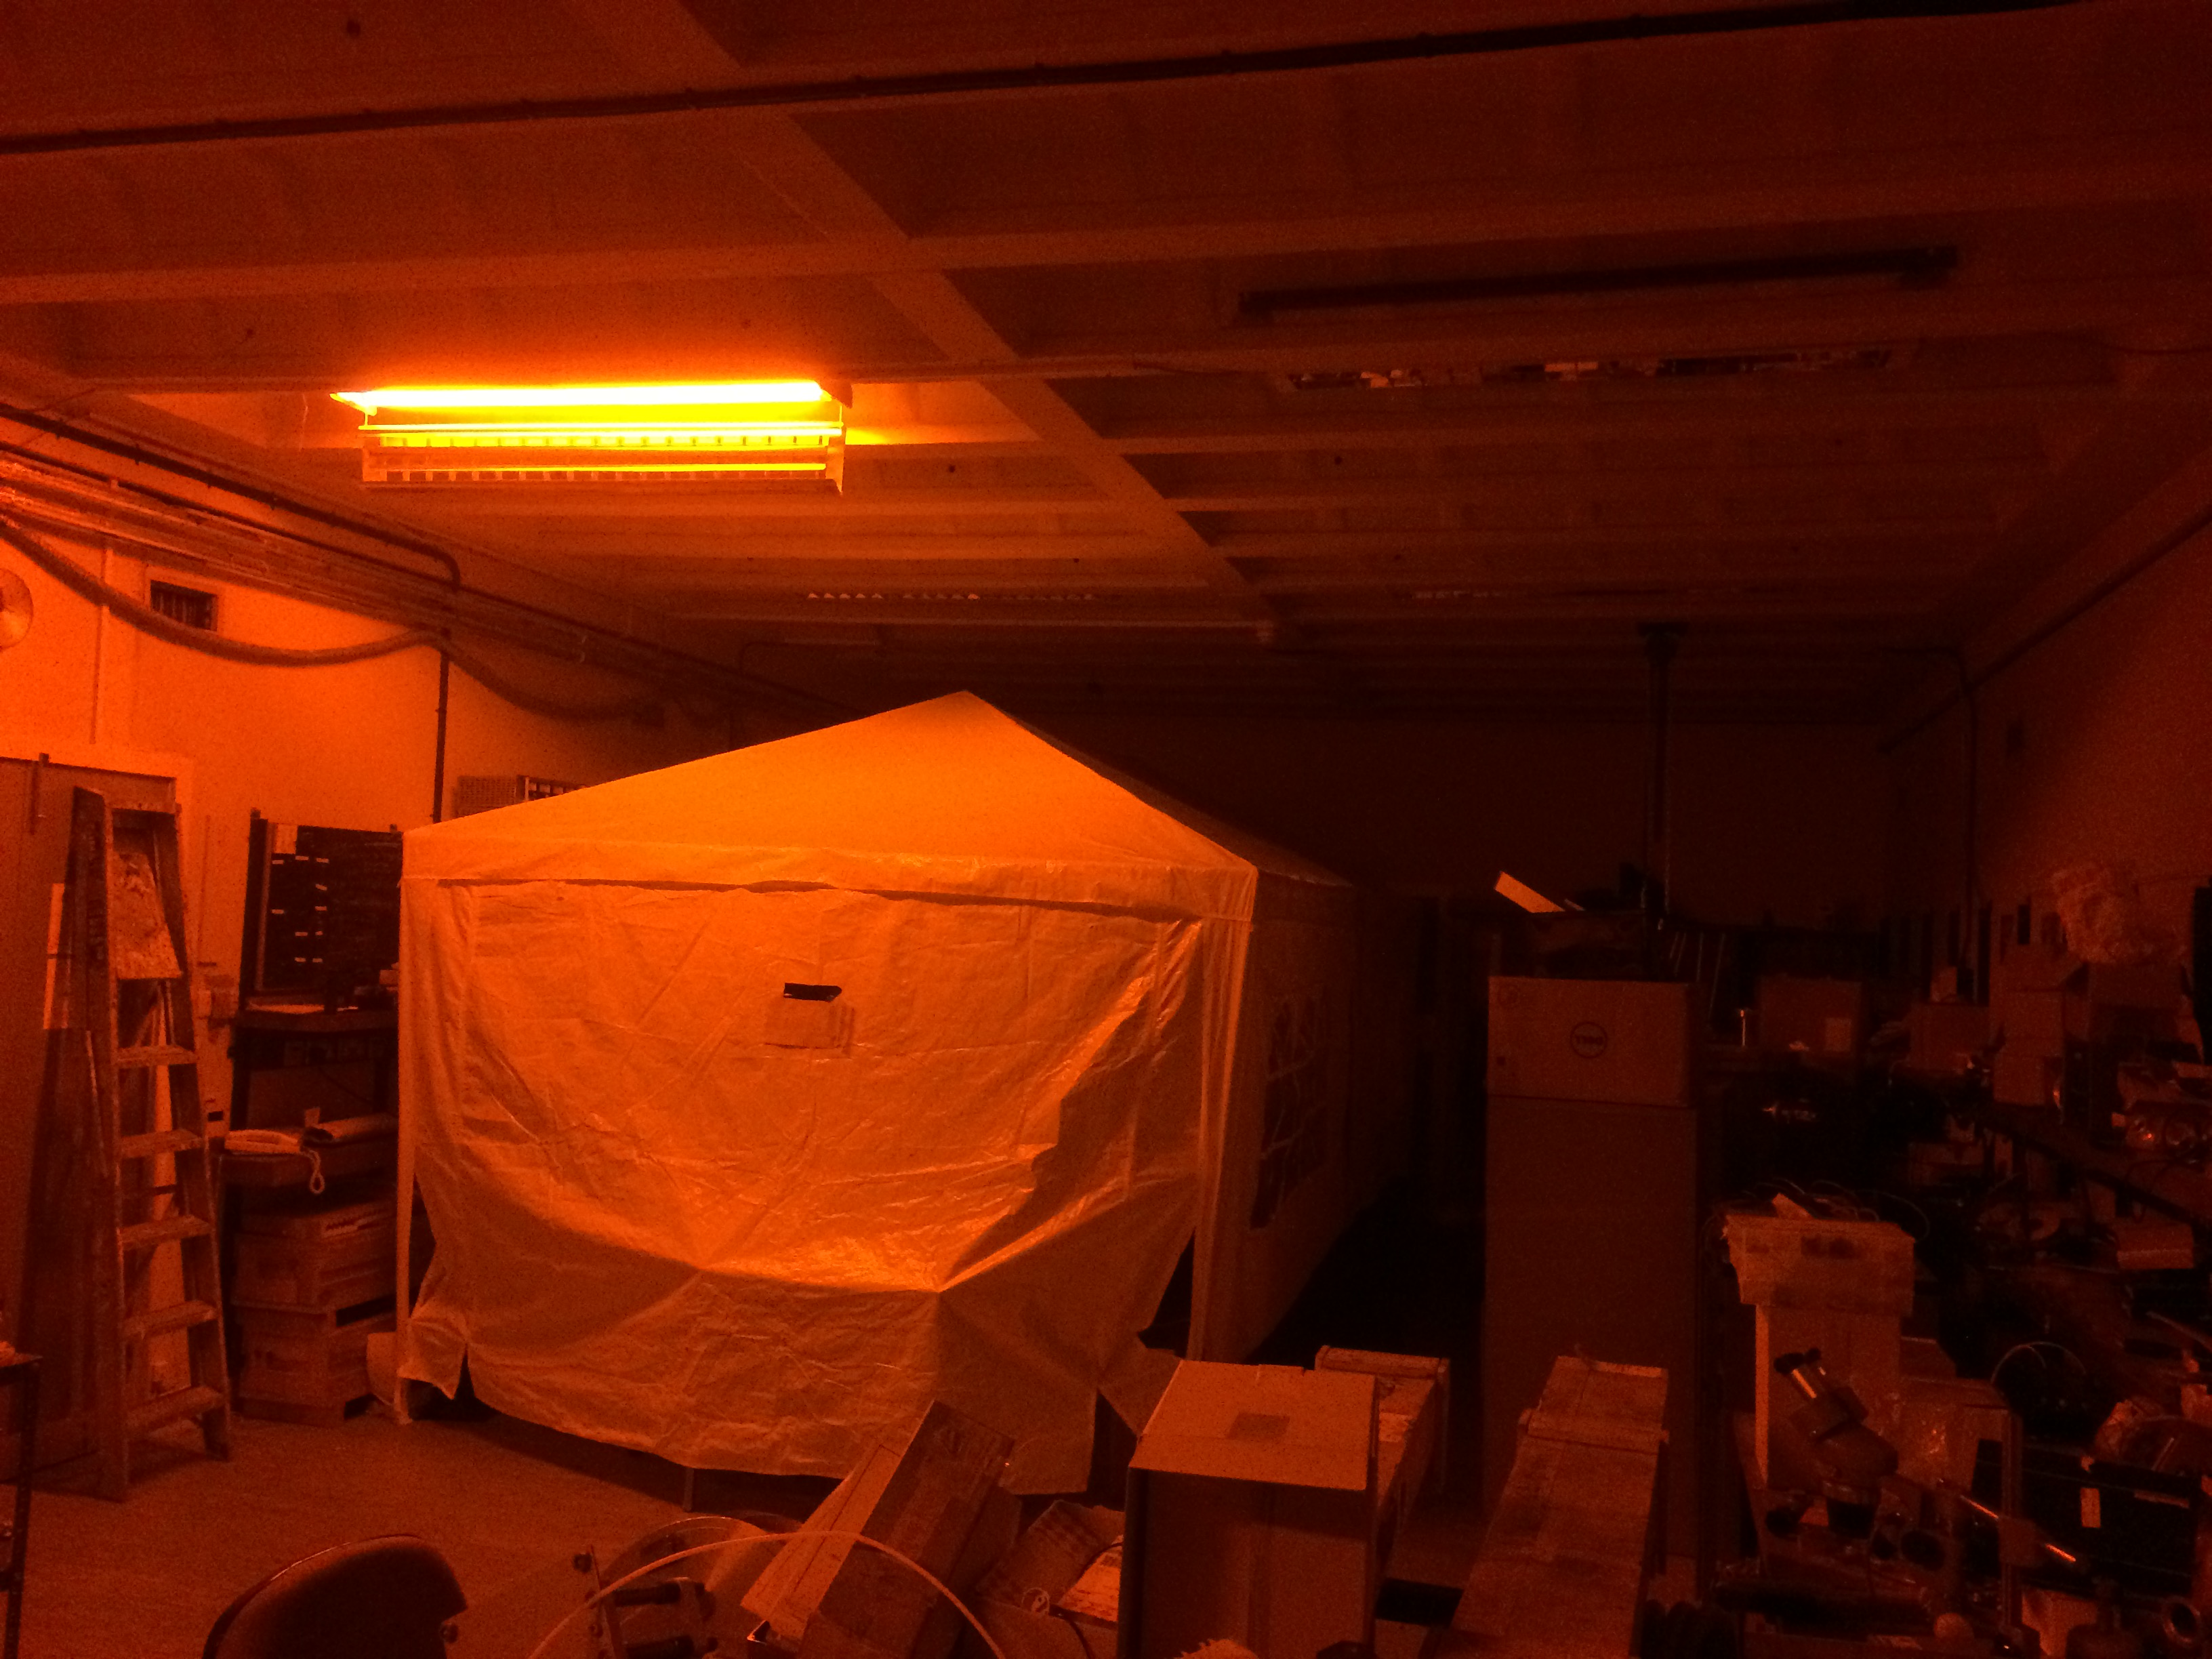
\includegraphics[width=0.7\textwidth]{ImgChap1/NoUV_setup1}
	\caption{A photograph of the laboratory used for the construction of the hodoscope.}
	\label{HodoTent}
\end{figure}


\subsection{Tile and Fibre Preparation}

A rigorous and meticulous approach to preparing each of the individual tiles and fibres was critical to the absolute performance and consistency accross the many different channels of the detector. Initial testing was of the tiles and fibres was carried out on a small sample of the larger order supplied before the major order that allowed the preparation process to be optimised.

\subsubsection*{Tile Preparation}

The plastic scintillator tiles were cut  to size and polished by the supplier before being outsourced to a specialist firm to drill the channels for the wavelength shifting fibres. All the tiles dimensions were measured and each carefully inspected for signs of crazing or any other damage with any damaged tiles excluded from use in the detector. This data was stored for future use in optimising the arrangement of the tiles in the detector. Initially a subset of these tiles were prepared to check the quality and consistency of the scintillator tiles, ensuring the performance of the detector. Once these checks were passed each tile was hand painted with 3 thin coats of Ti$O_{2}$ reflective paint. Brushing from the centre of each side towards the edge to minimise edge lapping. After painting each side was lightly sanded to produce a smooth finish. The width of the coat of paint was then measured at multiple points using vernier callipers, comparing to the tile dimensions previously collected. This is to ensure a thickness of 0.15-0.2mm for optimal reflective properties, without excessively increasing the dimensions of each tile. This process was repeated for every side of each tile and final dimensions collated for positioning optimisation. Where corrections were needed the painted sides were first smoothed with a layer of P1200 grade sand paper before refining the surface with $3\mu$m grade optical lapping film until smooth.

Small variations across a number of successive tiles can sum up to produced significant asymmetries and misalignments across the detector volume, hence the need for such meticulous control over this process. Figure \ref{elementgap} demonstrates the inherent gaps present within tiles, minimising these is critical to maintain the alignment and acceptance of the detector system.

\begin{figure}[!ht]
	\centering
	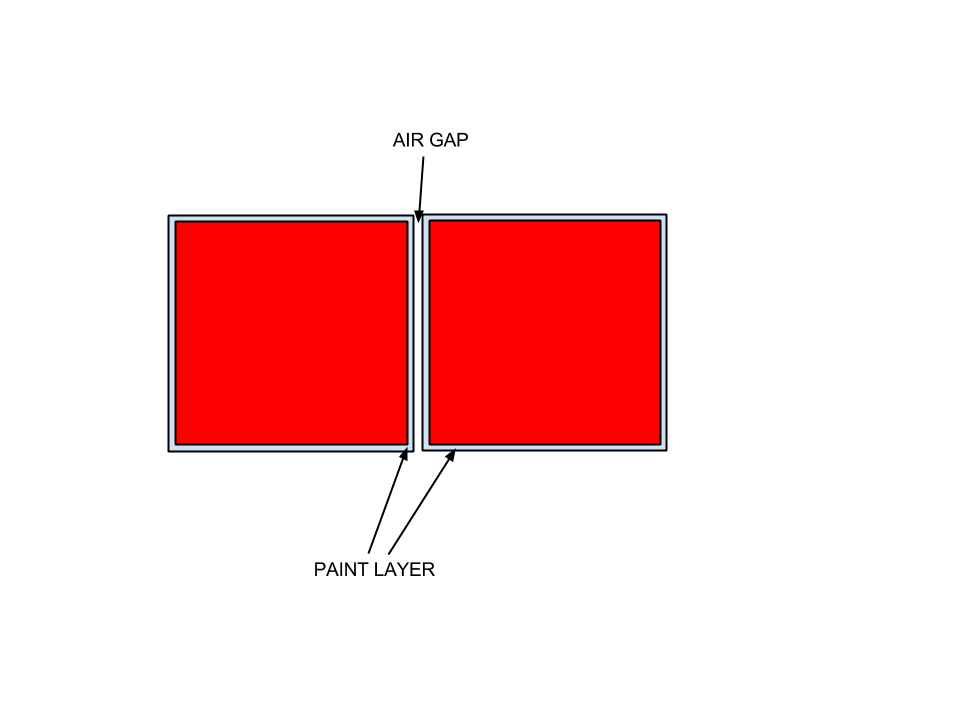
\includegraphics[width=0.7\textwidth]{ImgChap1/gap}
	\caption{Illustration of the inherent gaps present between tiles.}
	\label{elementgap}
\end{figure}

\subsubsection*{Fibre Preparation}

Once testing was successfully completed the major batch of clear and wavelength shifting fibres was shipped to Fermi Lab to be cut and prepared for fusion splicing. Each length of fibre was checked for any signs of damage before lengths of 6m of clear fibre were and 10cm lengths of WLSF were polished using the Ice Polishing method \cite{gallas1998polishing}, before being fusion spliced together with the join protected by a protective jacket. The 1 mm diameter fibres were then put into groups of 4 and slid into protective 3mm diameter black PVC sleeving which acts to protect the fibres from damage and seal it from outside sources of light. The final stage of the preparation process was to put a reflective mirror the WLSF end of the spliced fibres. Each end was cleaned using a lens cloth and Isopropanol (IPA) solution to remove any dust. Two thin coats of $TiO_{2}$ were then applied to the end of the fibre and any excess on the sides remove with IPA. The mirroring must reach the very edge of the fibre to effectively reflect the majority of light which is carried near to the edge of the fibre. However it must not exceed the boundary or the fibre will not fit into the channels in the scintillator tiles.


Cleaning, polishing, inspection, consistency checking etc. Testing a subset of the fibre and tiles to ensure consistent quality of the finished product.
\cite{hanlet1999comparison}
\cite{gallas1998polishing}

\subsection{Assembly}

Once the elements were prepared the first stage of the assembly process was to arrange and glue the scintillating tiles onto the carbon fibre sheets that form the base of each layer of the hodoscope.

During construction the hodoscope was split into its two layers and each group of scintillator elements was arranged and affixed to their respective carbon fibre sheets separately before the two layers were combined for later stages of construction. A cross section through the side of the detector including the 4 carbons plates and the separating pillars is shown in Figure \ref{hodocrosssec}

\begin{figure}[!ht]
	\centering
	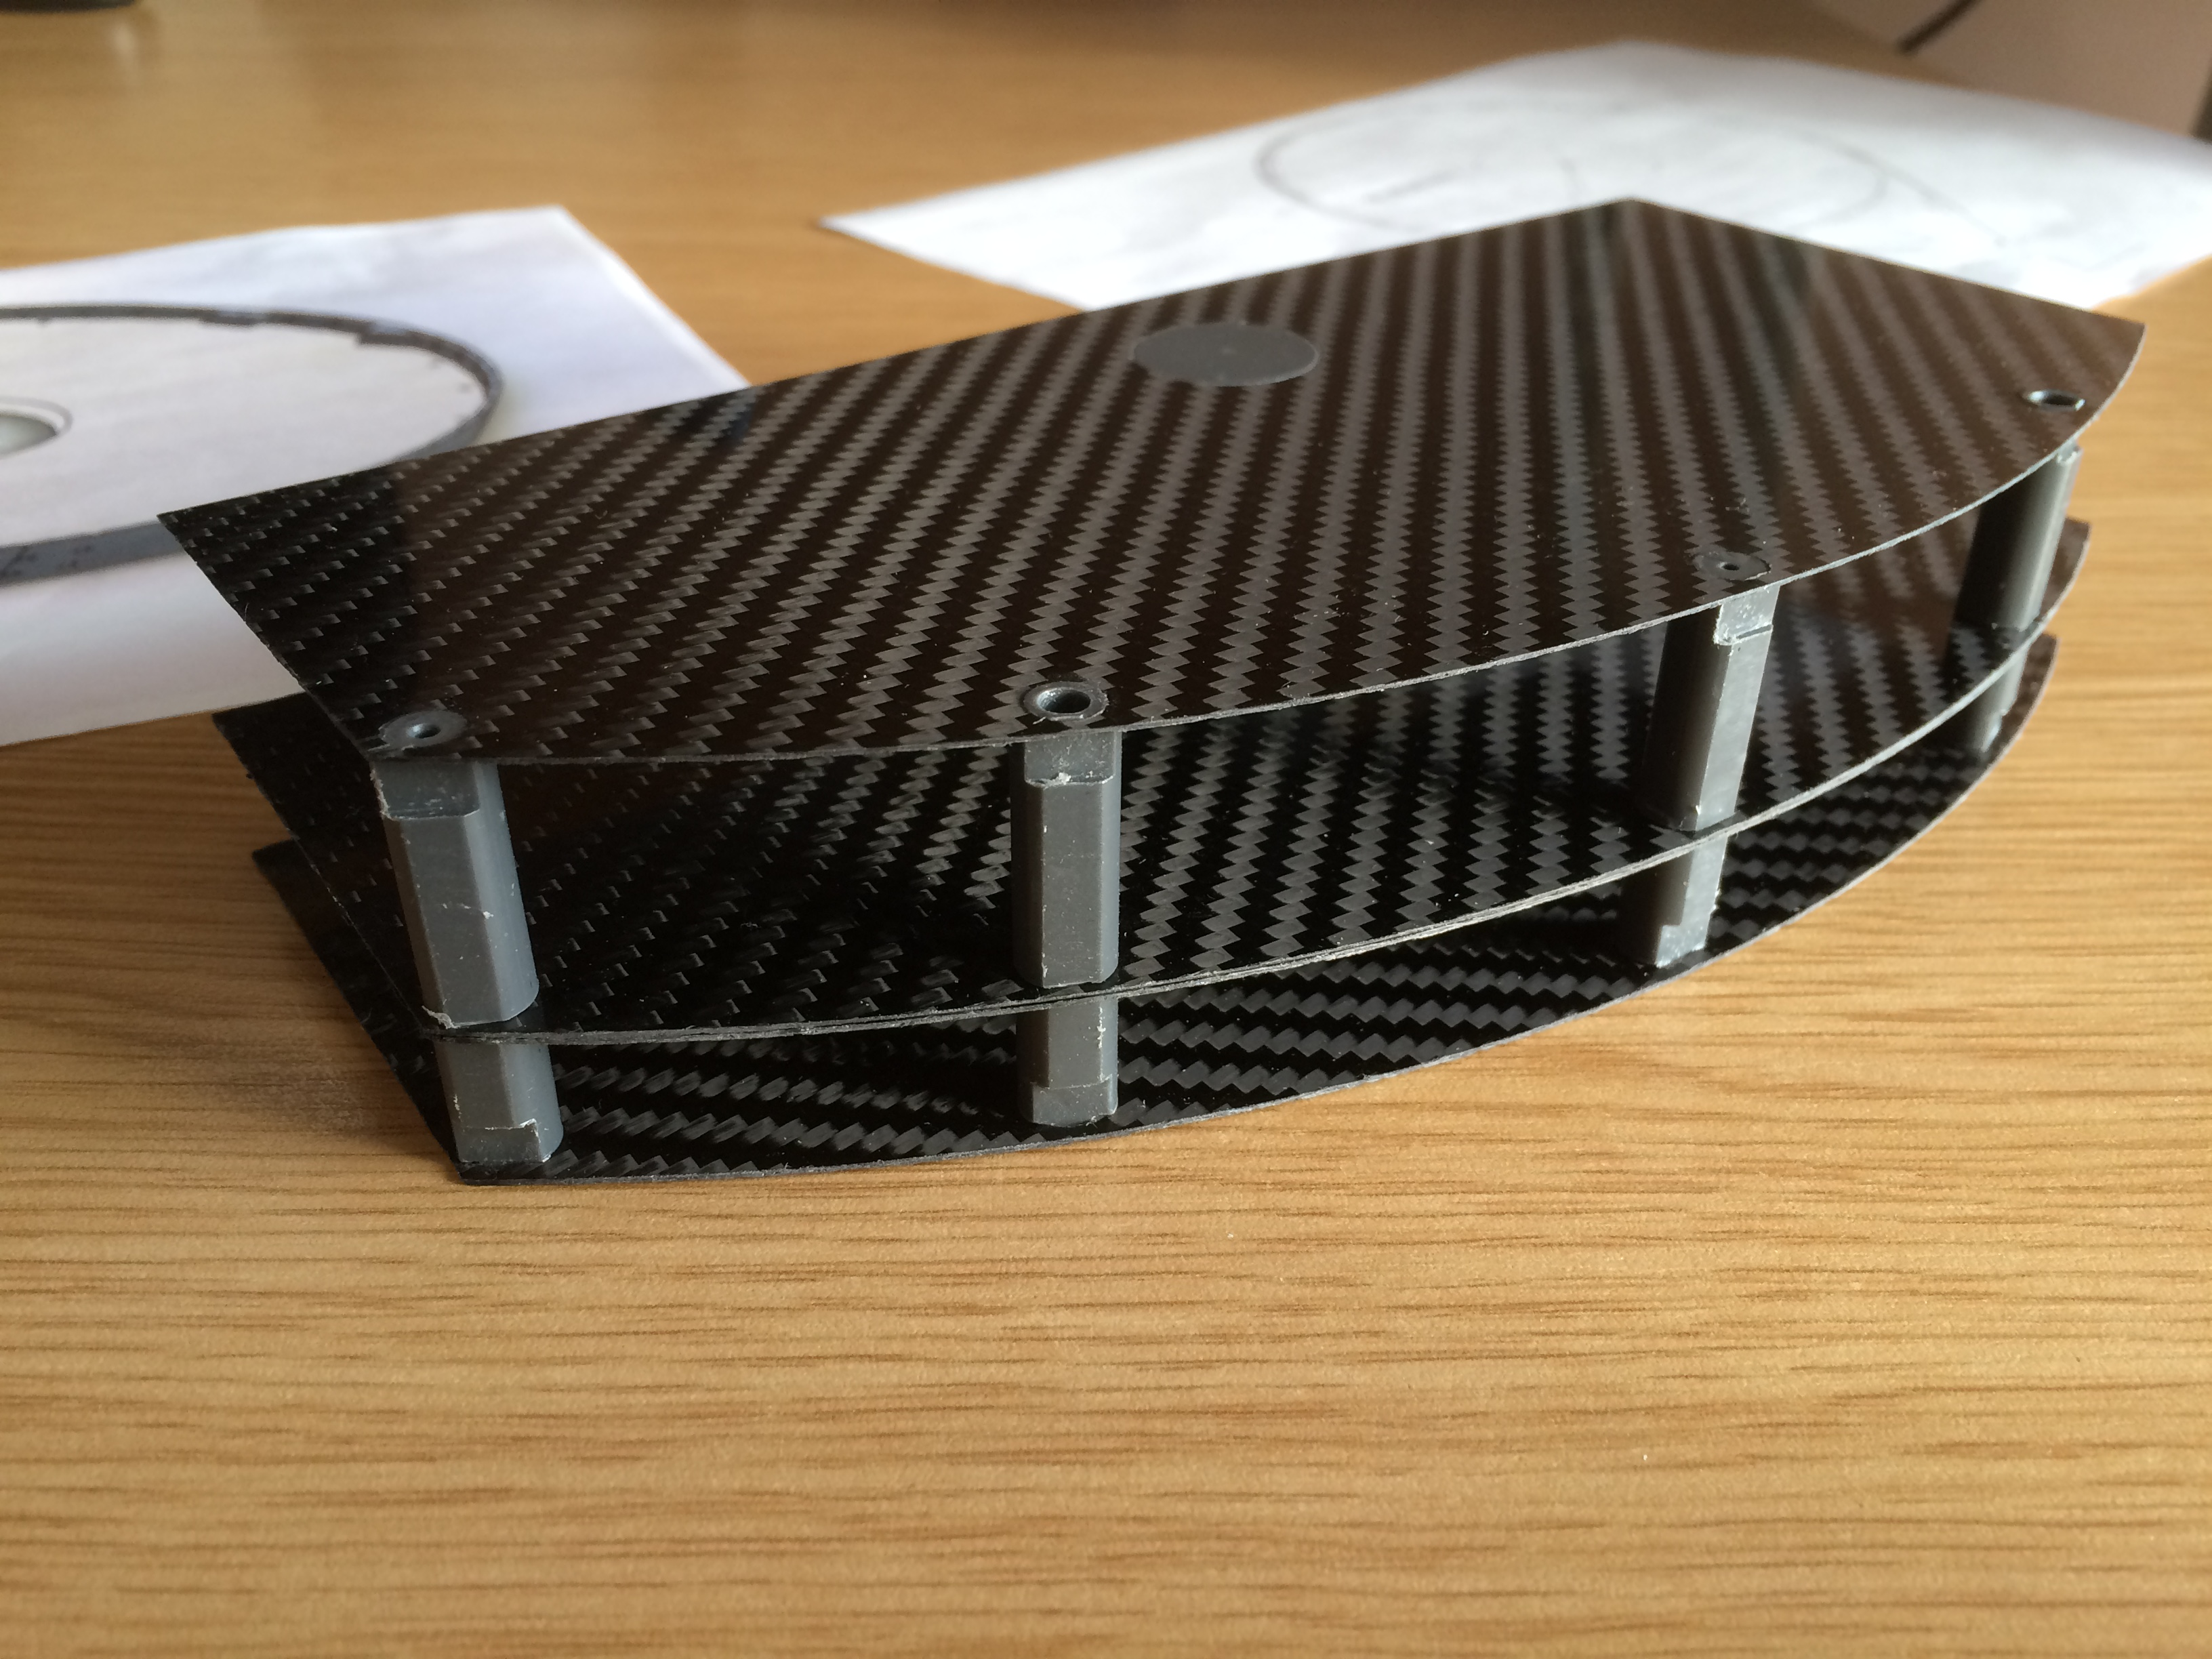
\includegraphics[width=0.7\textwidth]{ImgChap1/enclosure_hodoscope7}
	\caption{A cross section through a prototype of the hodoscope structure showing the carbon fibre plates and supporting pillars for the two layers.}
	\label{hodocrosssec}
\end{figure}

%\subsection{Component arrangement and Numbering systems}

\subsubsection*{Tile arrangement}

The tiles are cut to size to a tolerance of less than 0.1mm, however these small differences, particularly combined with further uncertainty introduced by the thickness and smoothness of the reflector, can create small but significant gaps between tiles. To maximise the acceptance of the detector an optimisation algorithm was written to arrange the detector tiles to minimize the gaps between them. It also prioritised the minimization in regions close to the beamline which are affected by a higher luminosity than the regions at higher scatter angles.

The regions most strongly affected by any deviation from the standardised size are those where several p15 tiles are grouped together, marked in blue in figure \ref{hodoelements}. In these regions there are twice as many tile edge then in a similar space filled with p30 tiles amplifying the affect of small differences. To compensate for these pressures. one p15 tile in the centre of each row of scintillators around the centre of the detector was cut slightly slimmer to maintain the uniformity of the detector tile arrangement. 

\begin{figure}[!ht]
	\centering
	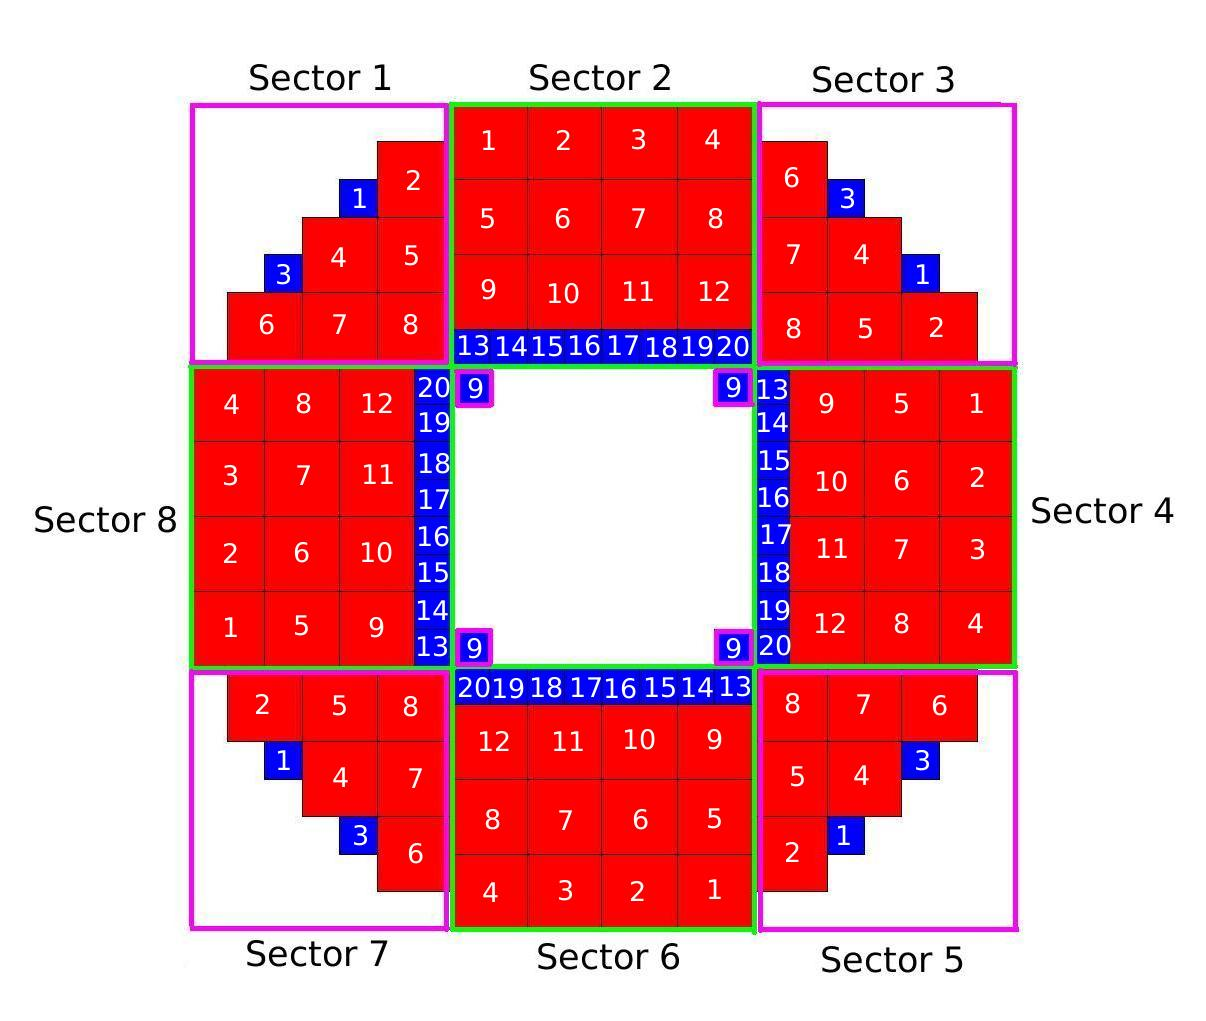
\includegraphics[width=0.7\textwidth]{ImgChap1/hodoelements}
	\caption{A schematic view of the scintillator tile arrangement in the hodoscope.}
	\label{hodoelements}
\end{figure}
	

The critical central P15 elements were positioned using a 3D printed pastic jig, positionally alligned by affixing to the central ring of the detector. Outside this the optimised P30 tile groupings of even sectors were positioned using a bespoke machined metal jig, the set-up is shown in Figure \ref{tilejig}. This configuration ensured orientation with respect to the tiles in the calorimeter. The critical P30 tiles closest to the centre of the detector, which are exposed to the greatest level of flux, were aligned first with the others progressing radially outwards in the jig. After this the odd sectors were added aligned by the even sectors already in place again working radially outwards in each sector. Finally the inner ring of P15 tiles were added to complete the arrangement.

\begin{figure}[!ht]
	\centering
	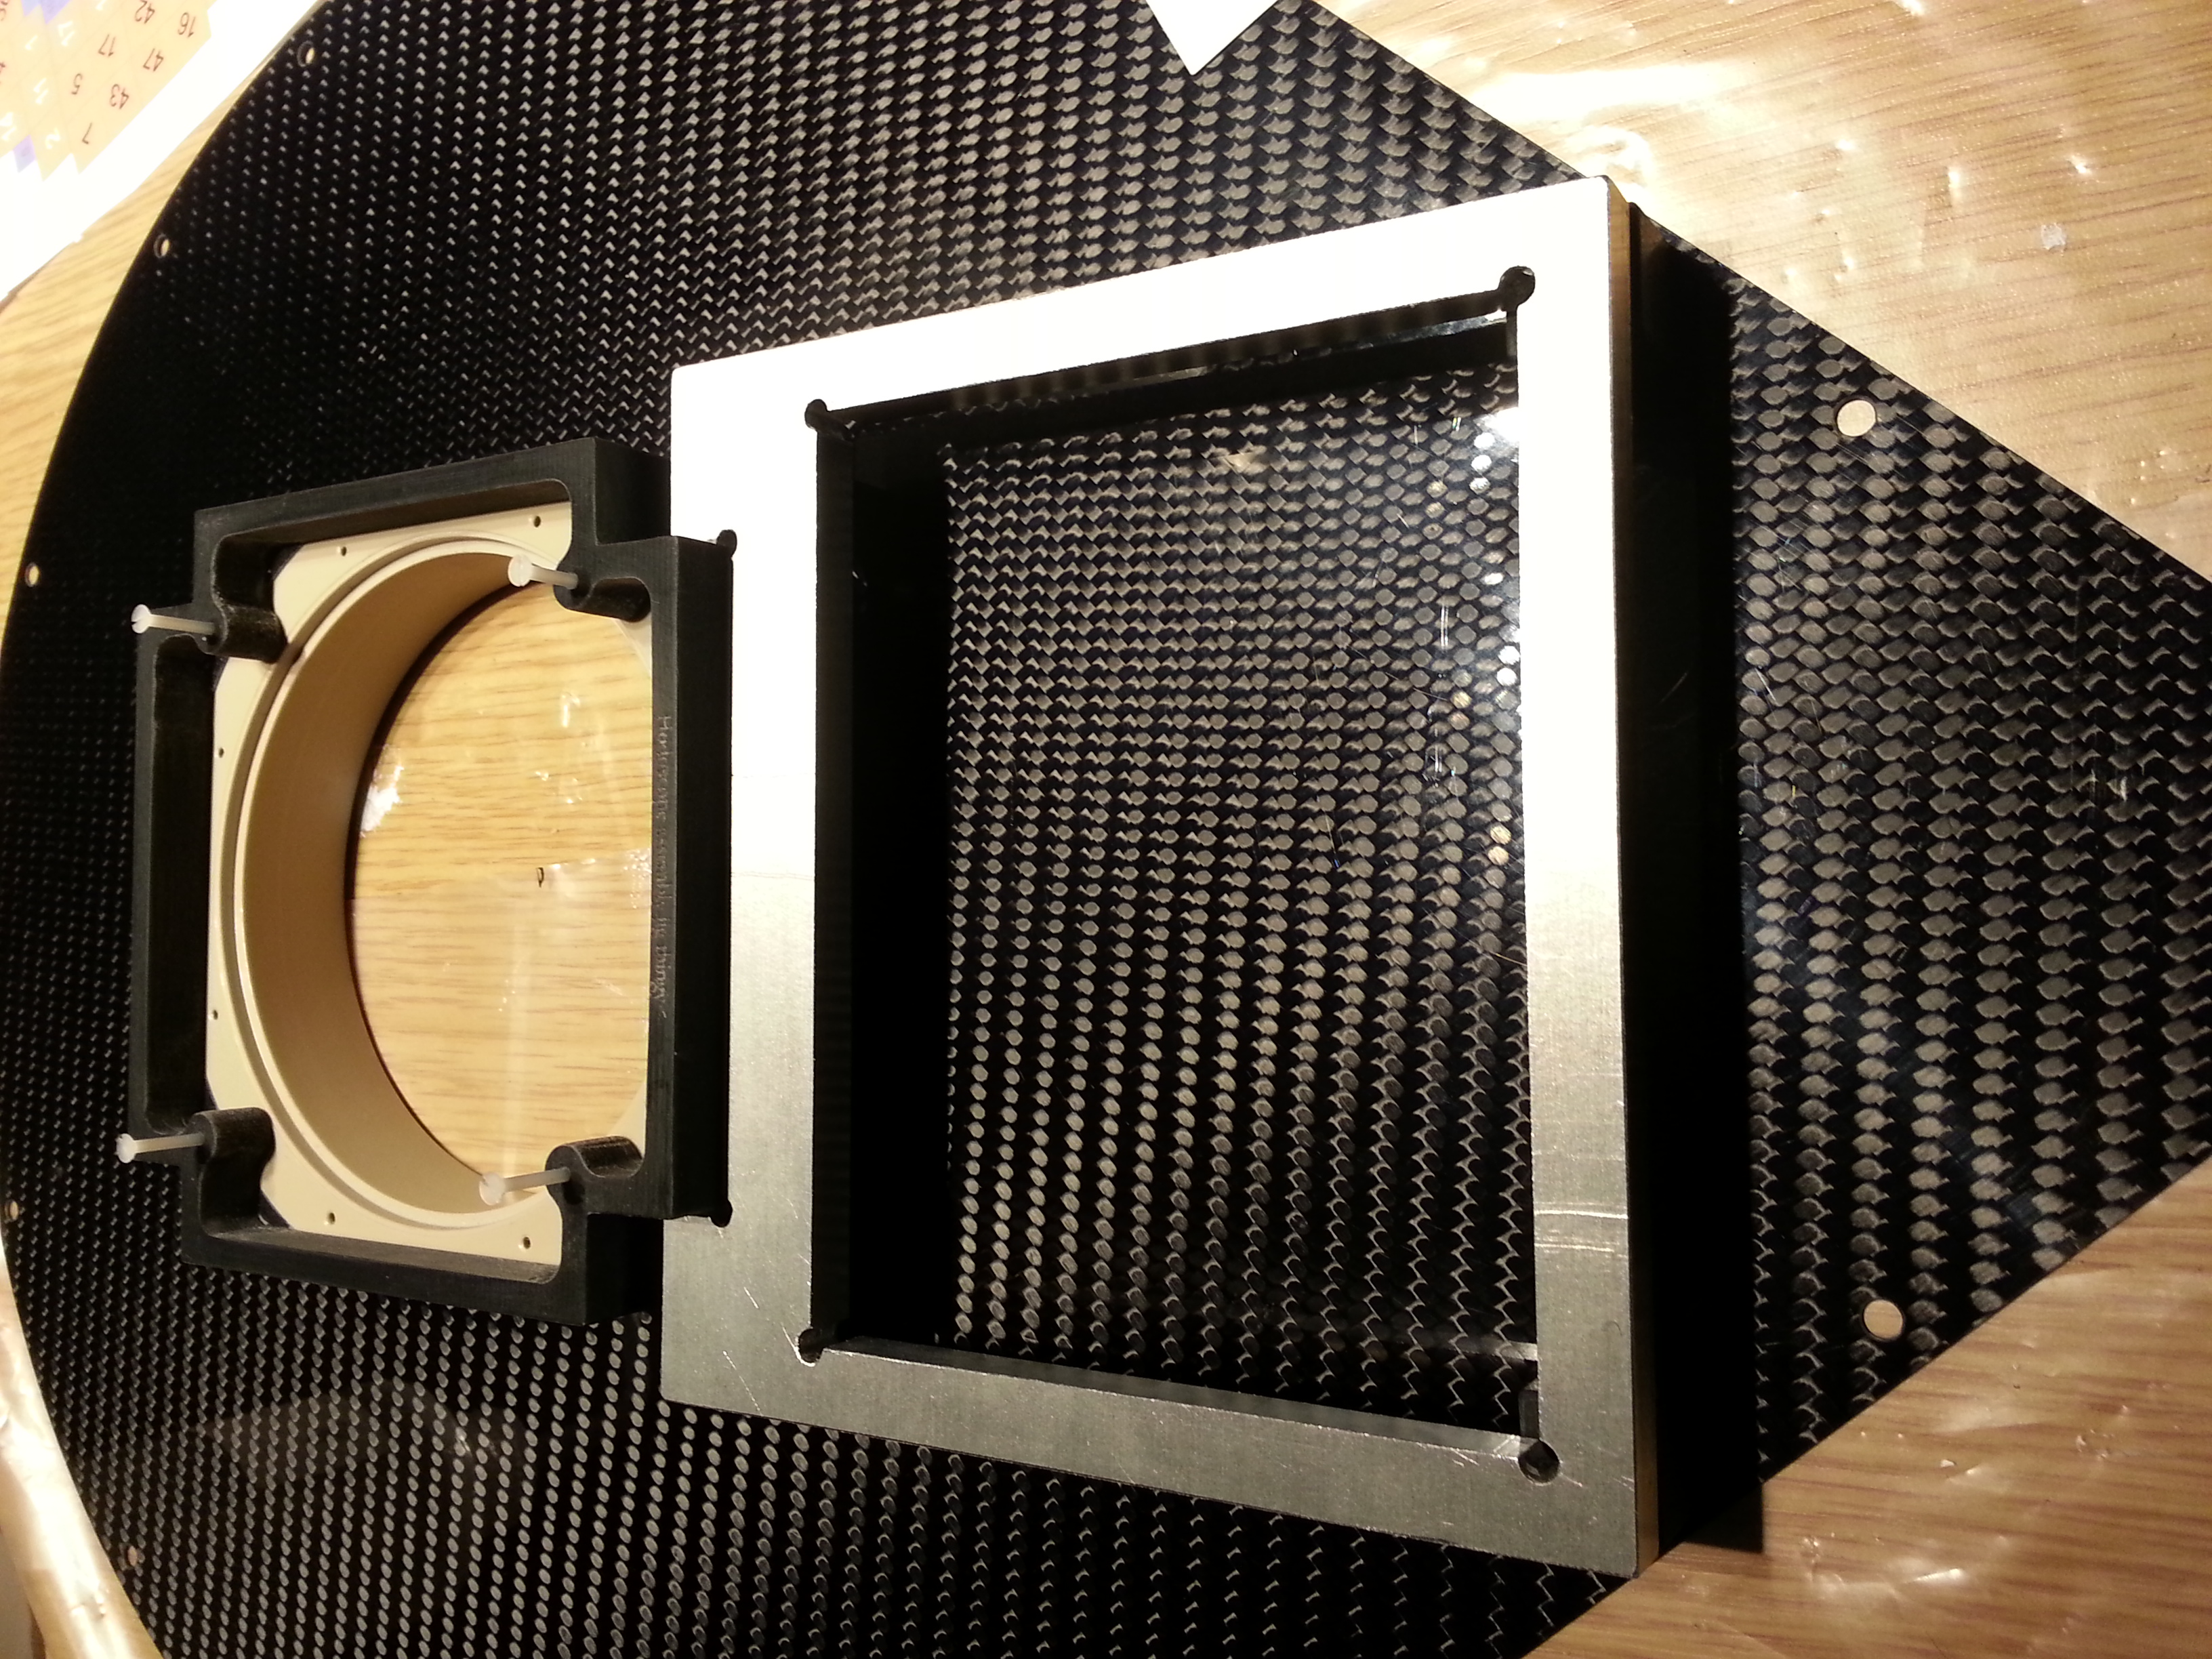
\includegraphics[width=0.7\textwidth]{ImgChap1/jig}
	\caption{A photograph of the plastic and metal jigs used to allign the detector tiles.}
	\label{tilejig}
\end{figure}

\begin{figure}[!ht]
	\centering
	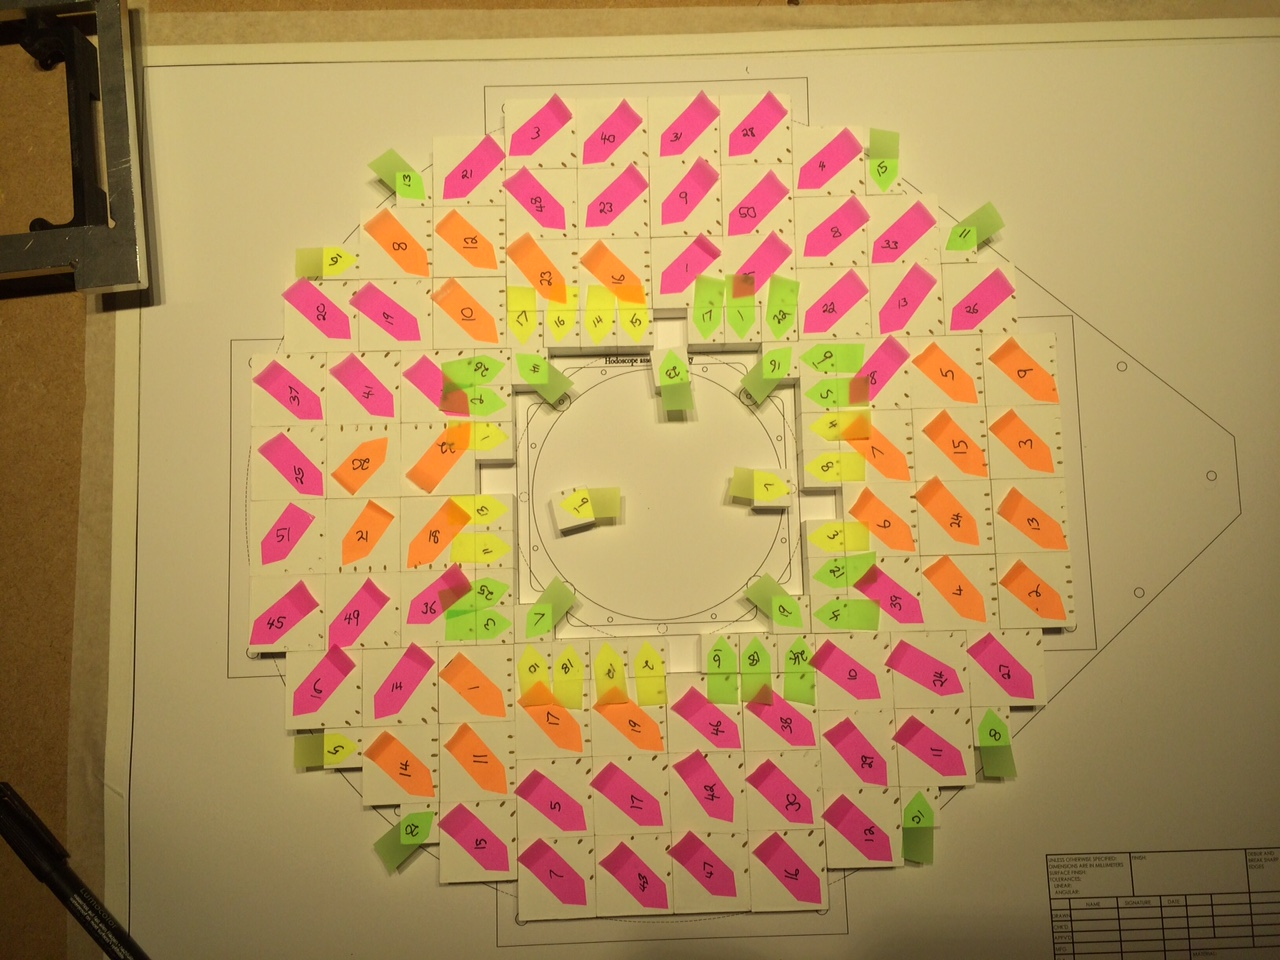
\includegraphics[width=0.7\textwidth]{ImgChap1/layout}
	\caption{The optimised configuration of tiles in position on the carbon fibre support plate.}
	\label{optimisedtiles}
\end{figure}

While optimising and quality control can minimize the affects of asymmetries propagating towards the edge of the detector in a design that attempts to maximise acceptance there will always be some. These can be clearly seen in Figure \ref{tileovershoot} with a limited number of tiles extending beyond the limit of the detector volume after positioning. These excesses were cut in the machine workshop in Edinburgh and the process of polishing, sealing and quality control repeating for the new edges.

\begin{figure}
	\centering
	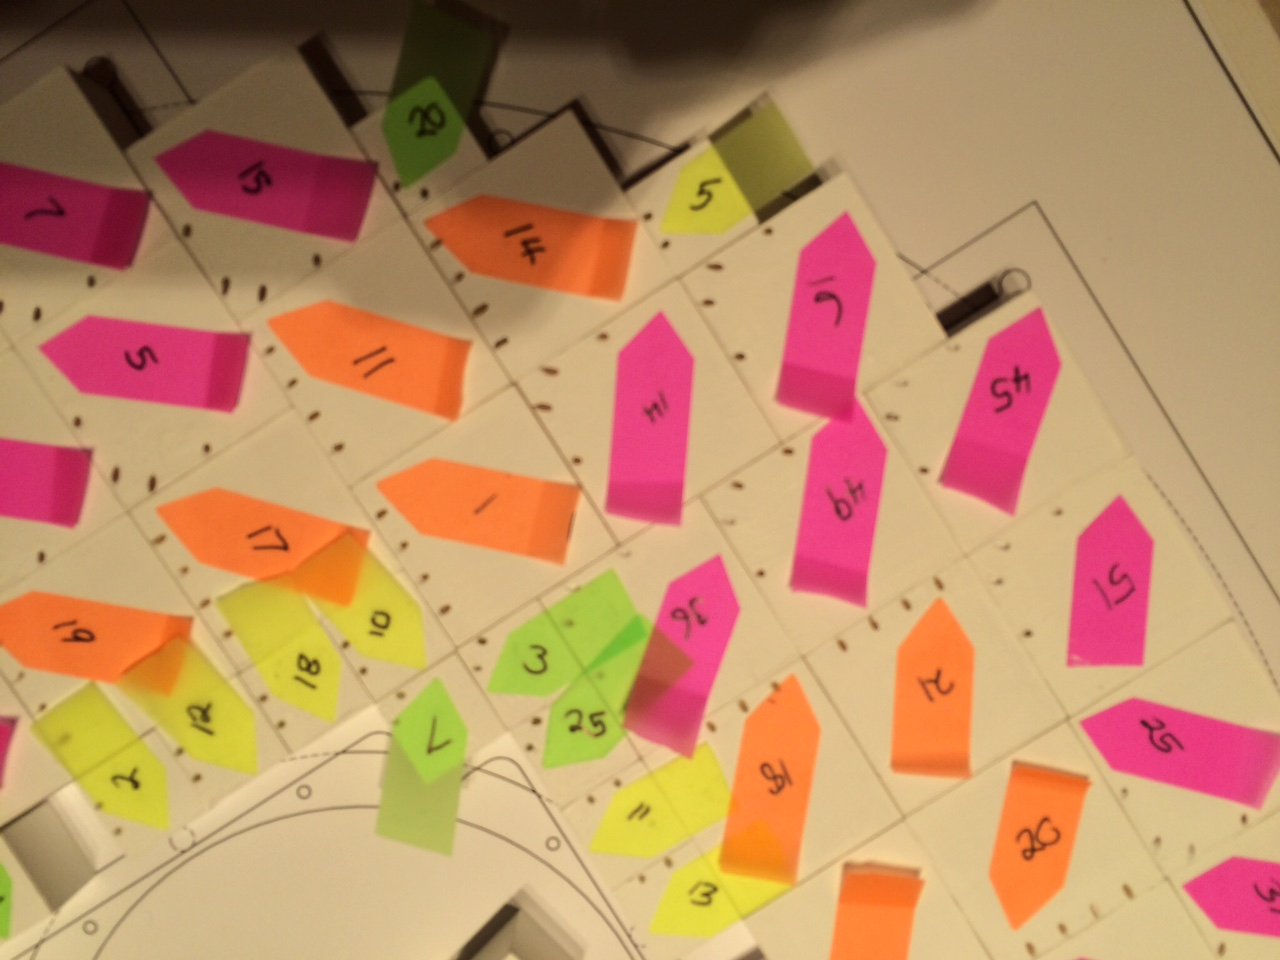
\includegraphics[width=0.7\textwidth]{ImgChap1/layoutzoom}
	\caption{An example of tiles purtruding over the radially limits of the hodoscope.}
	\label{tileovershoot}
\end{figure}

Once all tiles had been positioned and optimised each one was individually lifted using vacuum tweezers and glued into position using two part epoxy adhesive araldite that cured over 2 days. A slow curing Araldite was selected for its known radiation hardness and minimal impact on the tiles during the curing process. After gluing a foam back support layer was placed over the tiles with small weights to minimise the chance of movement during curing. Once all tiles were attached in place a precision survey was carried out to map all the tiles positions in relation to the central structure of the detector. The results of this will be critical when relating data taken from both layers of the hodoscope, along with the forward tagger tracker and calorimeter.


\subsubsection*{Fibre arrangement}
	
Fibre pathing throughout the main detector volume, through the transition into the confined space in the delta wing will be discussed in this section. There is limited space within the detector volume and a large number of fibres to route. As a result some compromise has to be made between ideal routing for each individual fibre, and the collective affect on the system. It is also critical that each scintillating element performs above the design requirements, so tiles which have more restricted pathing need to be prioritised to ensure their light output is sufficient.
		
When optimising the routing it is critical to consider a number of factors
	
\begin{itemize}
	\item Tiles further from the delta wing have more flexibility for routing.  
	\item There is a tight limit on the vertical height between the tiles and the roof of the detector volume. 
	\item Minimising cross over between fibres helps to improve packing efficiency.
	\item Certain tiles cannot be routed to the nearest exit points because it would require too tight a bending radius.
	\item The critical point for the fibre exit is the juncture at the base of the main volume at the edge of the final row of tiles. Where the maximum number of fibres have to fit through a limited space. 
\end{itemize}
		
Considering these factors and testing arrangements with prototypes in the laboratory, lead to the grouping shown in Figure \ref{FibreGrouping}. With 12 groups of 4 bundles with 4 fibres in each one, for each half of each layer, with a mirrored arrangement in the opposite half. 


\begin{figure}
	\centering
	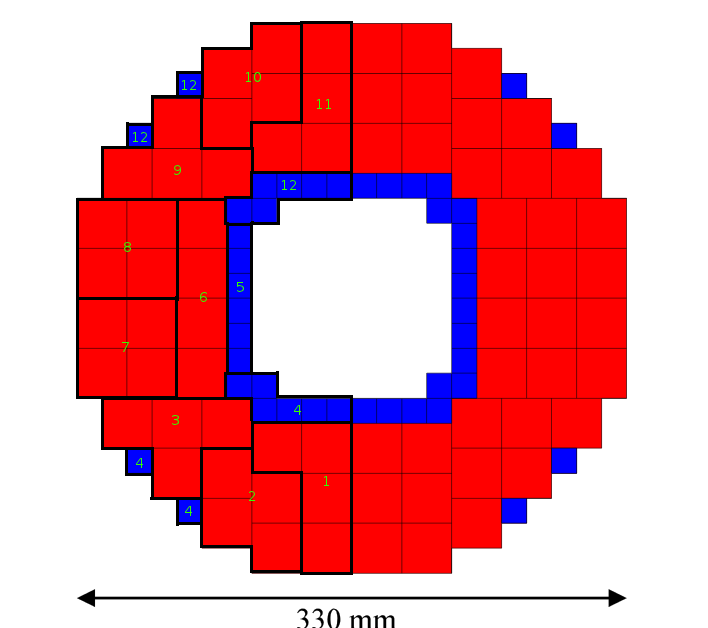
\includegraphics[width=0.7\textwidth]{ImgChap1/groups}
	\caption{The groups of tiles allocated to different columns in the hodoscope delta wing. Column numbers ascend from the closest point to the central pillar in the delta wing outwards towards the edge. The arrangements are mirrored symmetrically for both sides of the detector and apply to both the thick and thin layers.}		
	\label{FibreGrouping}
\end{figure}

Each group was allocated a column in the delta wing, numbered from the centre outwards, with the closest elements to the delta wing filling the lower rows of the columns. In groups which included p15 tiles, which only have 2 fibres per element, 2 tiles were routed into the same fibre bundle. This was essential was space management in the delta wing, and the fibres could be split again to separate SiPM channels upon reaching the electronics. The fibres from tiles further back from the delta wing tended to take a wider arc closer to the edge of the detector, leaving additional room for the densely packed fibres emanating from the p15 tiles at the centre of the detector. 

The bundled fibres in the delta wing are held in place with elasticated cords that pass around each collumn of 4 bundles, though holes at the base of the delta wing and are tied in place at the top of the delta wing. Each collumn of bundles is fixed in place at 2 points and the points shift along the length of the delta wing to minimize the space taken up by the cords. A photograph of the tied bundles pre-trimming of excess is shown in Figure \ref{deltacord}.

\begin{figure}
	\centering
	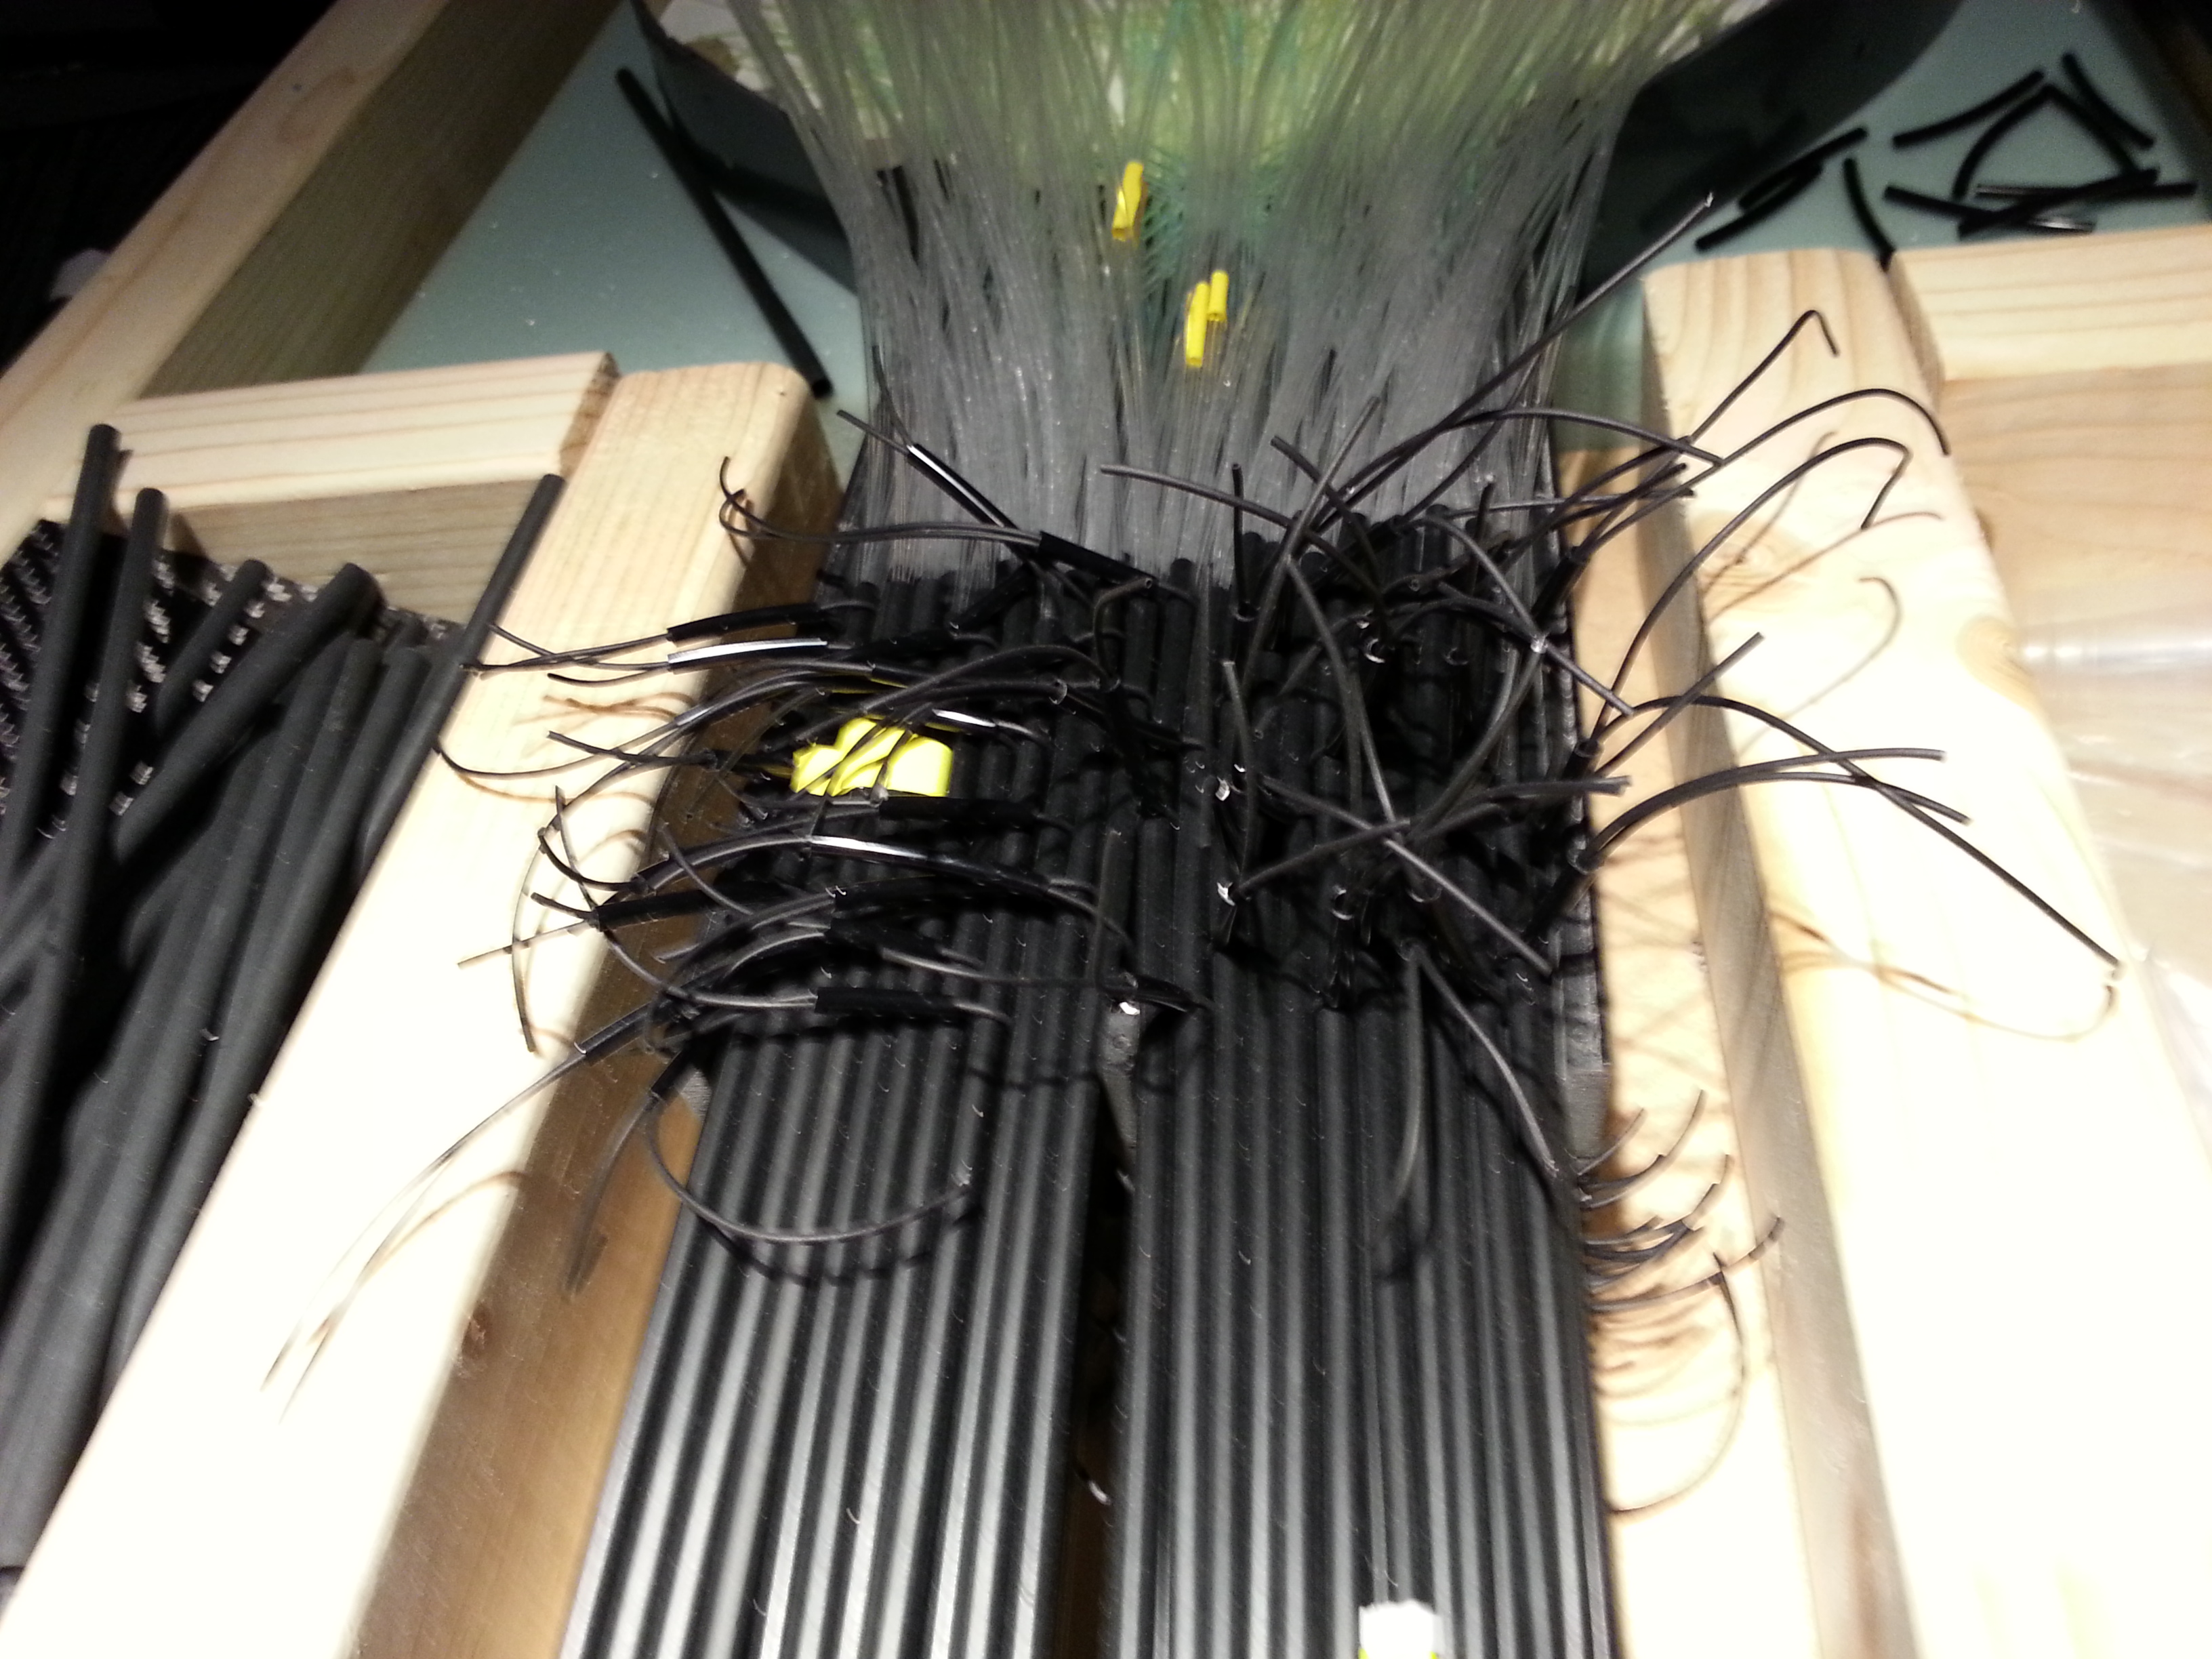
\includegraphics[width=0.7\textwidth]{ImgChap1/deltacord}
	\caption{The fibre bundles fixed in place in the delta wing.}		
	\label{deltacord}
\end{figure}

			
			
			
			
%In the delta wing and going into the electronics unit.

%Measuring the sizes of each tile to optimise the arrangement through the detector and minimise any gaps, maximising the effective coverage and this acceptance of the detector system. Focusing on the areas of highest flux where detector acceptance is most critical to be near perfect.

%Arranging the position and orientation of the tiles to maximise the efficiency of the fibre packing to minimise the vertical space taken up by the fibres and reducing and pressure load on the fibres. Identifying any critical areas of strain and how to deal with these pressure points.

%Arranging the fibres to fit into bundles, then how they would path through the detector, fit into the delta wing and transition through CLAS to reach the electronics.

%Arranging the bundles on the way to the electronics. The bundles must fit through tight space requirements, where maximising packing efficiency is critical. The fibres must be kept protected from damage and sealed from any outside sources of light or crosstalk.


			



			
\subsection{Gluing} 
			
Once the scintillator tiles were alligned and affixed into position for each of the layers in the hodoscope. The next stage in the consuction process was embed the WLS fibres into the channels in the tiles, following the fibre pathing design taking each fibre through the detector body and into position in the delta wing. This required affixing the fibres into place in a specific order, addresing problematic tiles as a priority and then progressing from the tiles closest to the delta wing moving back up the detector and radially outwards.

The optical glue used to fix the fibres into place was \textbf{GLUE NAME}. A radiation hard clear optical adhesive with a similar refractive index to both the scintillator tiles and WLS fibres. \textbf{GLUE NAME} is a two part adhesive that requires an overnight cure to solidify. The ratio of the components of the two part glue was accurately measured by first measuring the weight of the more viscous component of the glue being mixed on scales accurate to 0.01g. The secondary component was then added by a fine syringe up to the total weight for the exact ratio. The two part where then mixed with a mixing baton for 5 minutes following a figure of eight pattern to evenly mix the components. The combined glue was then placed in a vacuum chamber to remove any air bubbles that had been trapped in the mixture and visually inspected for consistency.

Once the glue was prepared, the tile channels were cleared of any debris using pressurised air before a small quantity of glue was inserted using a syringe directly into the very bottom of each channel. The lengths of fibre to be inserted were given a final clean with IPA, before being inserted one by one into the channels. Insertion of the fibres forced the pooled glue upwards forcing any in the channel up and out of the channel ahead of the glue and creating a smooth even connection between the fibre the the scintillator tile. Once glued in position the fibres were left raised up, so gravity ensured the fibres stayed in position filling the entire length of the channels. Tiles were glued in small batches to ensure ideal conditions for curing. 

The fibres also needed to be glued into the fishtale connectors forming the junction with the SiPMs to ensure a stable connection. In this case the glue joint is not an optical connection and the Araldite glue that was also used for affixing the tiles to the carbon sheets was the proffered option. The fibres for each element were inserted into the channels in the end pieces of the fishtale connectors leaving an overshoot of at least $\sim$5cm. The exact amount was dependent on the fibre path length between the specific tile and SiPM being used for each channel. A small ammount of glue was then applied to a $\sim$2cm lenth of this overshoot next the the connector and this was pushed back into the connector block for curing overnight. Once cured the fibres were trimmed using fibre cutters to before being polished flush with the edge of the connector. The fibres were then smoothed using several grades of optical lapping film down to 3$\mu$m for improved optical transmission. Figure \ref{postgluefishtale} shows the ends of the polished fibre connectors, with the green fibres of the open half of the hodoscope clearly visable. 

\begin{figure}
	\centering
	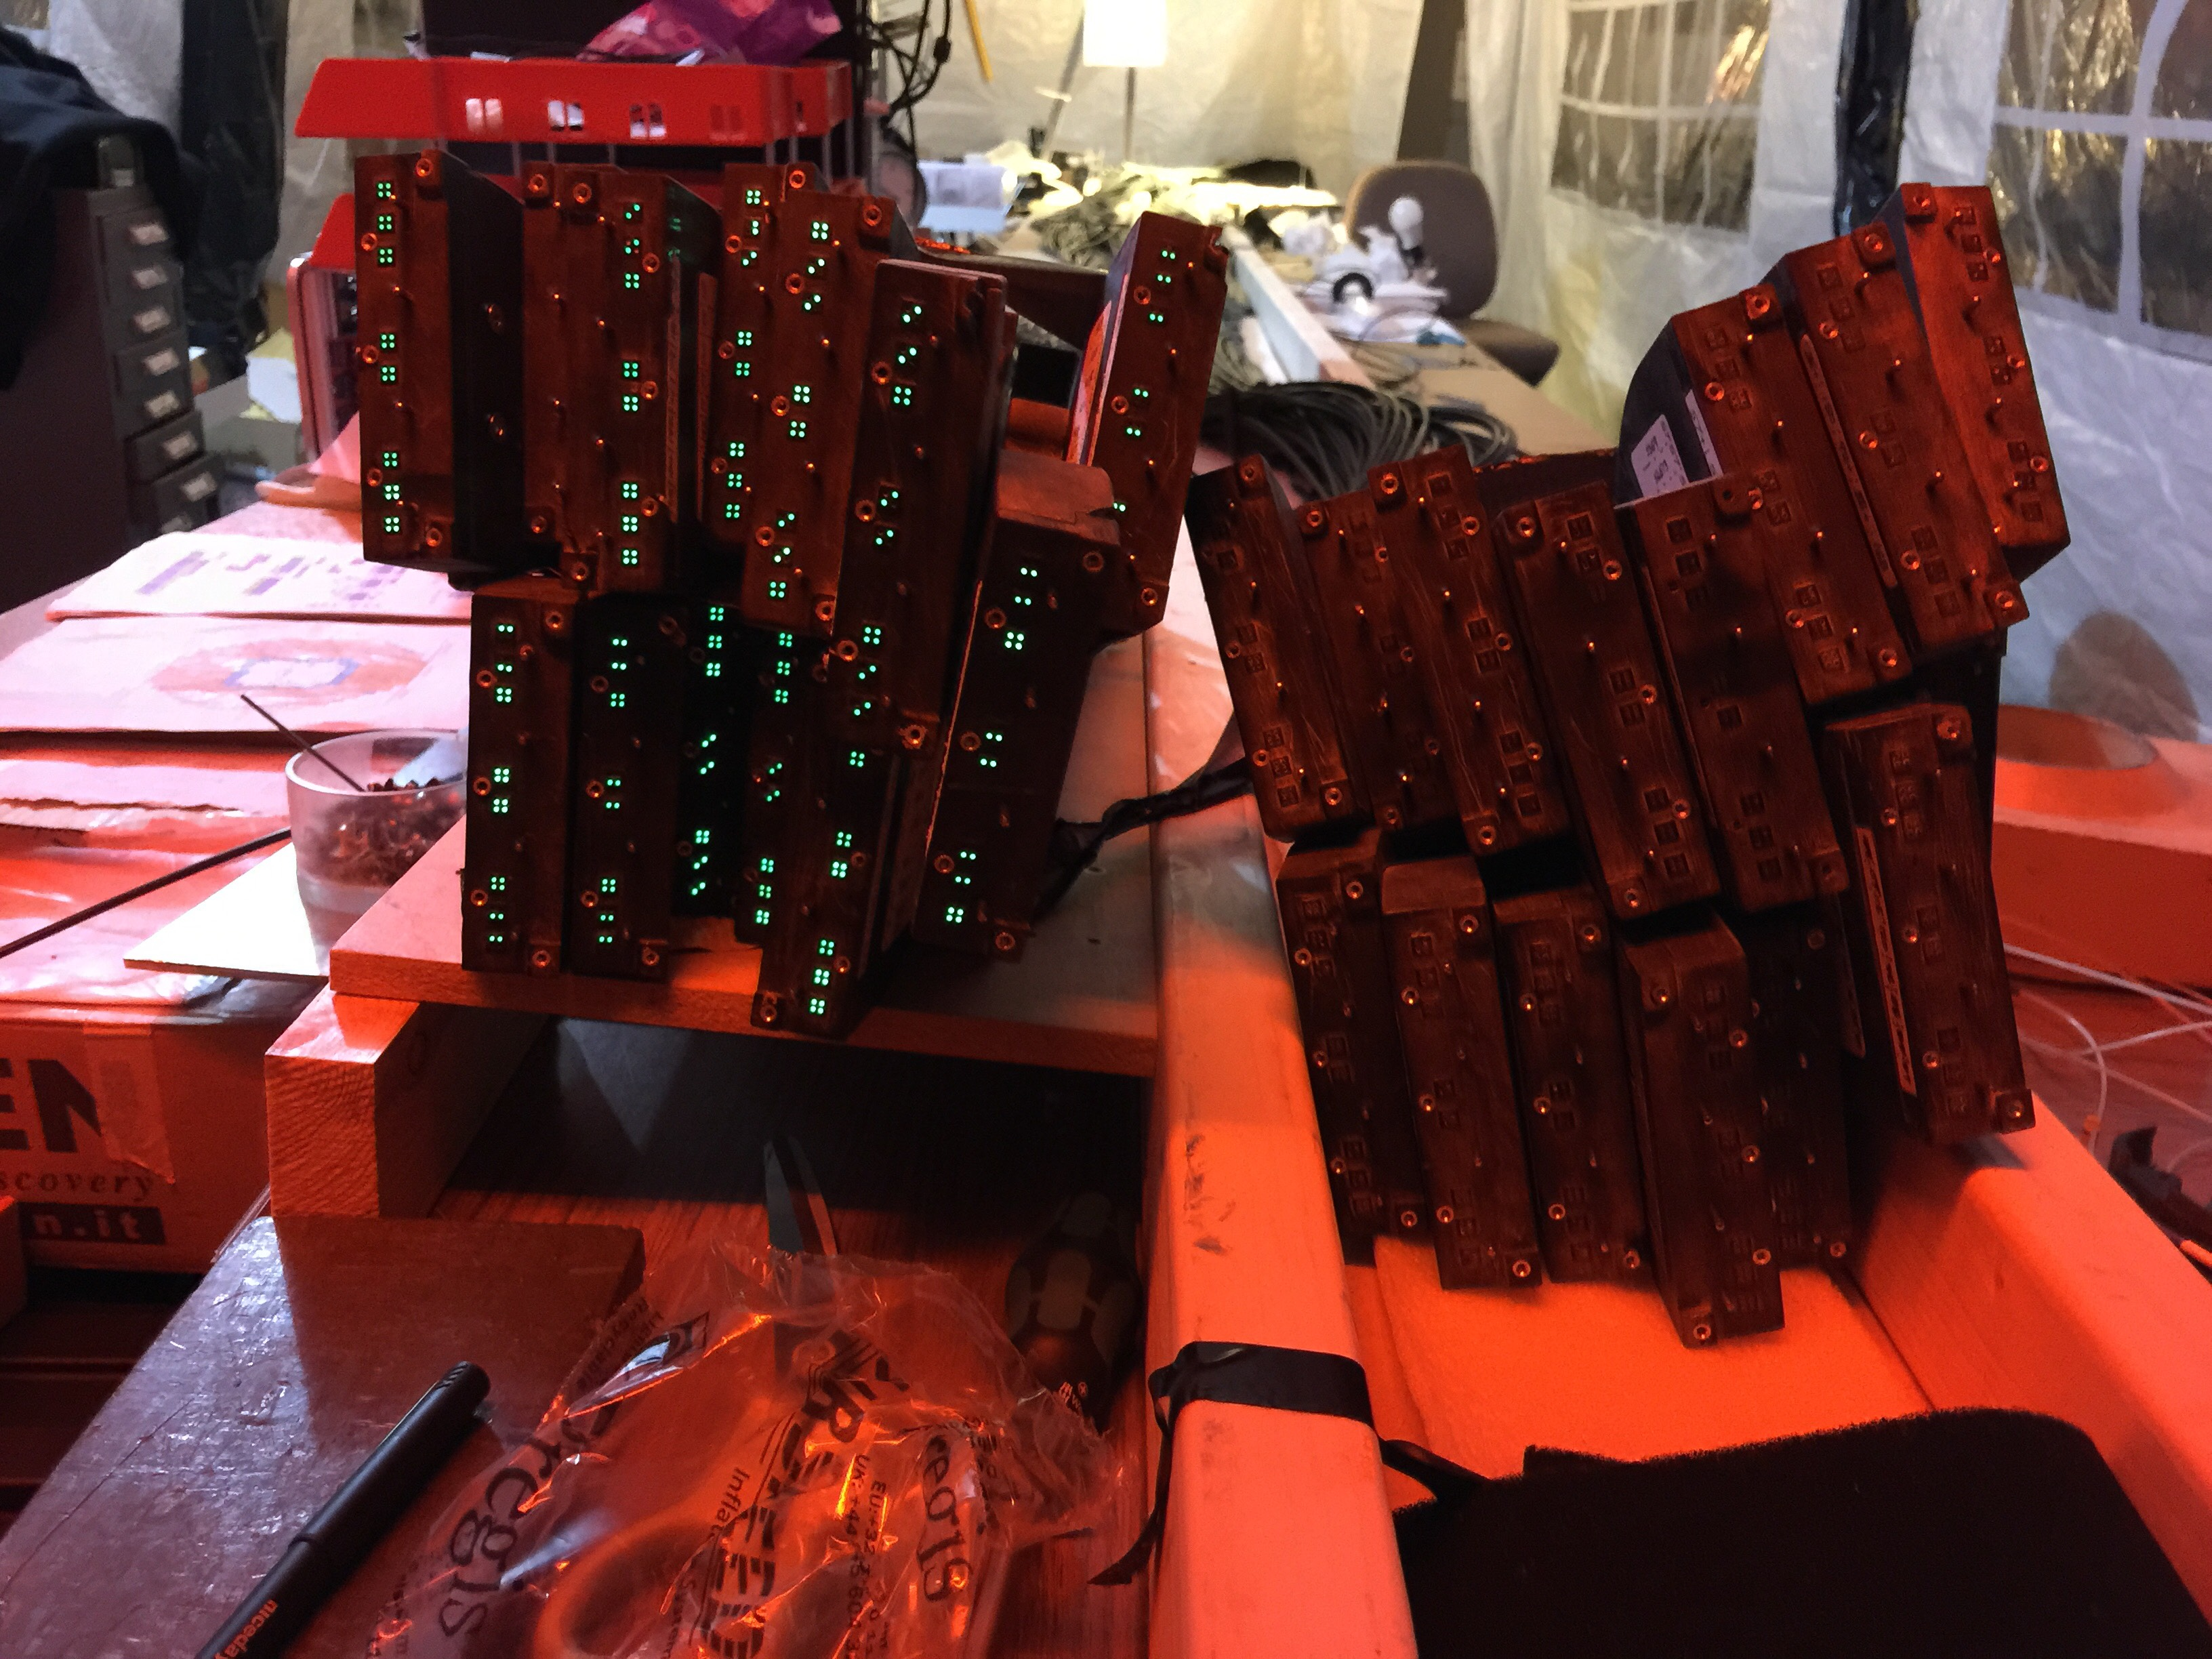
\includegraphics[width=0.7\textwidth]{ImgChap1/postgluefishtale}
	\caption{Ends of the fishtale connections after the fibres were glued into place the polished. The connectors from the layer of the hodoscope that is currently open are clearly differentiated by the captured green light than is radiating from the end sof the connectors.}		
	\label{postgluefishtale}
\end{figure}



			
%Different types of glue. 
%
%Studies on their transmitivity properties, effect of radiation damage, pot life (too fast and too much heat that will damage the fibres and tiles).
%
%Precise scales and pipettes used to ensure quality and consistency of the mix. Mixed thoroughly and then put under vacuum to remove any air bubbles.
%
%Glue inserted from the base of the channel forcing air out of the channel towards the top.

% something IPA used to clean all elements of any debris before gluing.

%Different glues used for holding the fibres in place in the delta wings and affixing the fibres into the tiles.

\subsection{Sealing the detector system}

Ensuring the detector system is sealed from external sources of light is integral the opperation of the detector system.

\begin{figure}
	\centering
	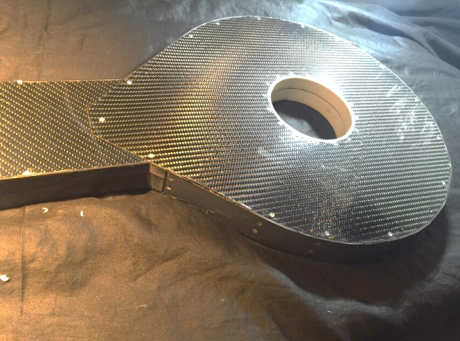
\includegraphics[width=0.7\textwidth]{ImgChap1/sealed}
	\caption{The sealed head of the detector.}		
	\label{sealedlollypop}
\end{figure}

\subsection{Packing for transport}

Bespoke designed structures was developed to secure and protect the detector while it was transported to Jefferson Lab.

\begin{figure}
	\centering
	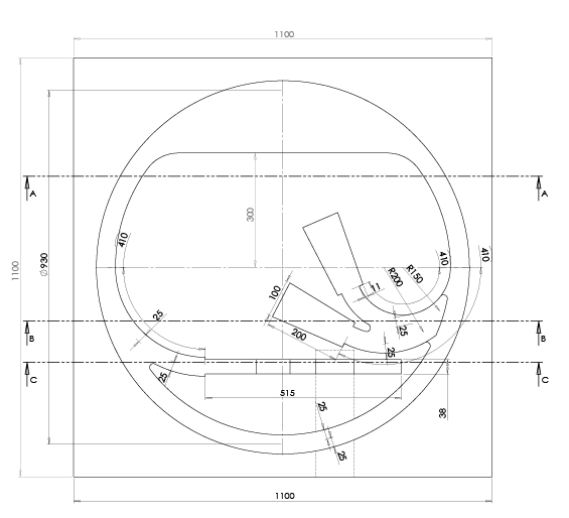
\includegraphics[width=0.7\textwidth]{ImgChap1/packing}
	\caption{The design of the packing crate of the FT-Hodo.}		
	\label{packing}
\end{figure}

\begin{figure}
	\centering
	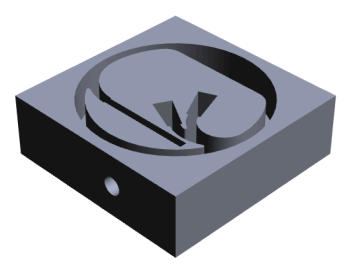
\includegraphics[width=0.7\textwidth]{ImgChap1/packingCAD}
	\caption{A CAD picture of the packing crate of the FT-Hodo.}		
	\label{packingcad}
\end{figure}

\begin{figure}
	\centering
	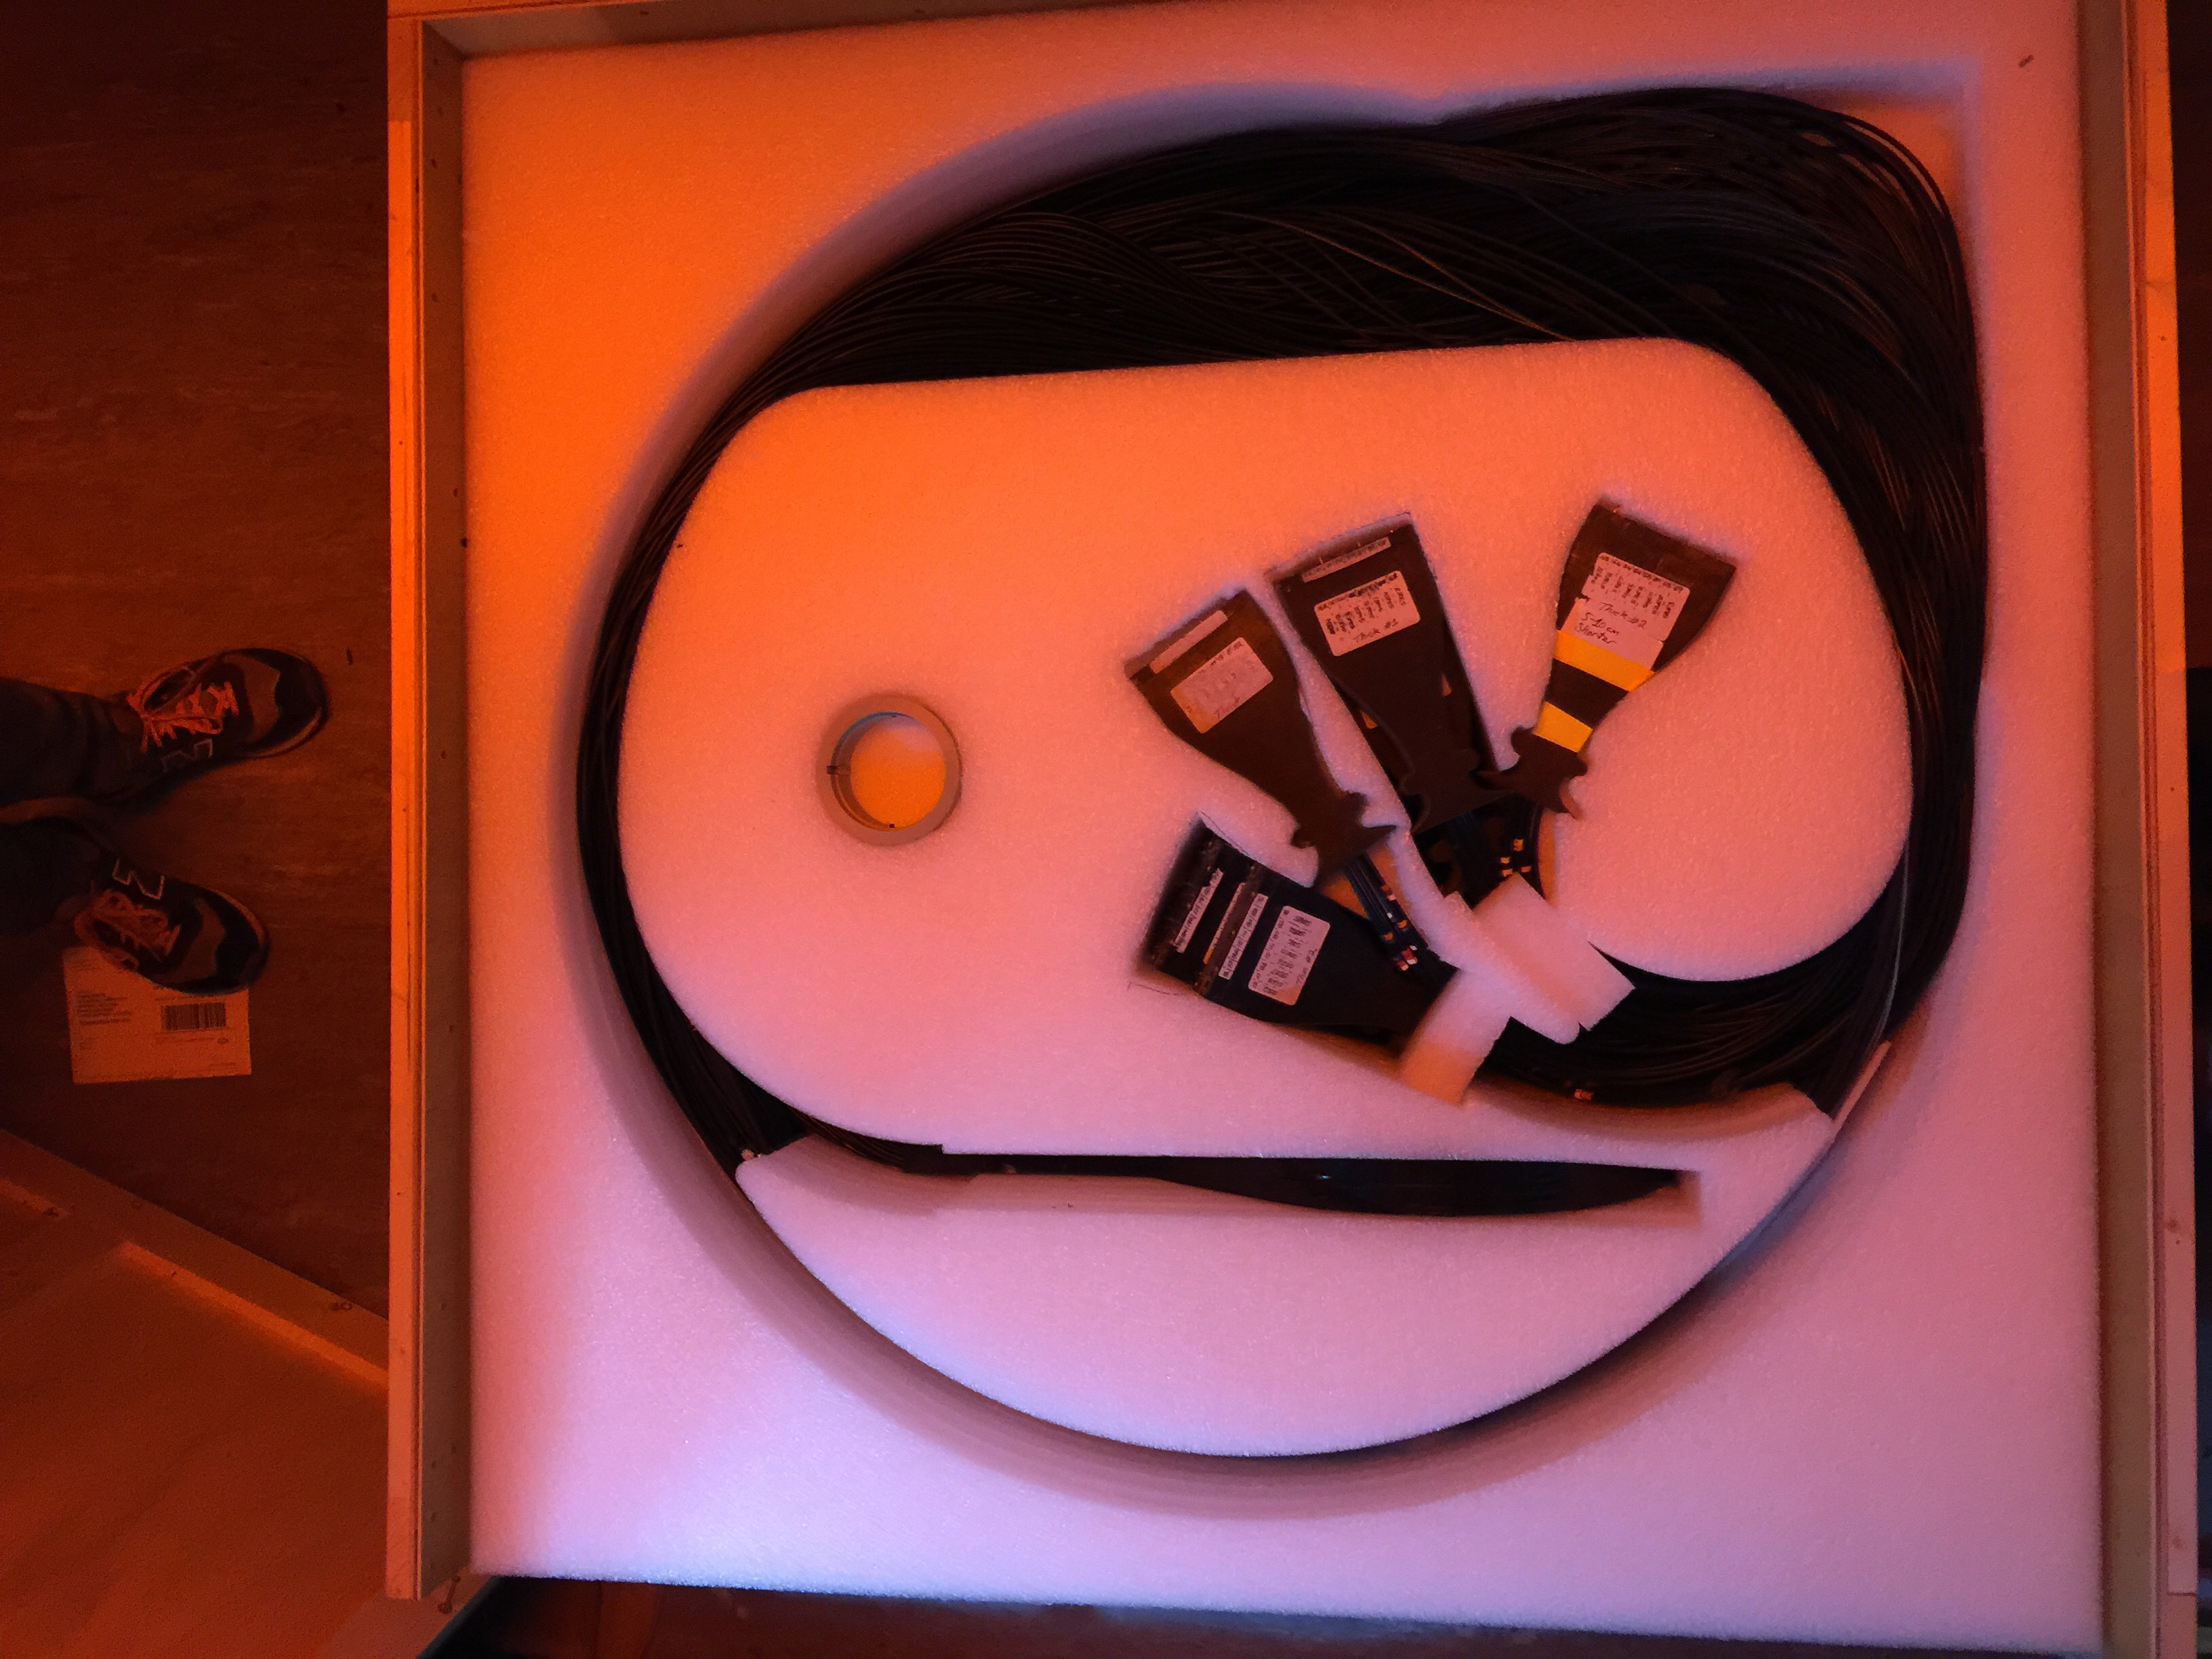
\includegraphics[width=0.7\textwidth]{ImgChap1/detectorpacked}
	\caption{A photograph of the FT-Hodo packed before being sealed and transported to Jefferson Lab.}		
	\label{packedphoto}
\end{figure}



\subsection{Testing at JLAB}

Construction completed in Edinburgh.

Transported to Jefferson Lab to begin further testing with the calorimeter in January 2016.

Setting up, configuring and continuing calibration of the detector system.

\begin{figure}
	\centering
	\includegraphics[width=0.7\textwidth]{ImgChap1/JLABTestingSetup}
	\caption{Setting up the hodoscope for testing at Jefferson Lab.}		
	\label{JLABSetup}
\end{figure}

\begin{figure}
	\centering
	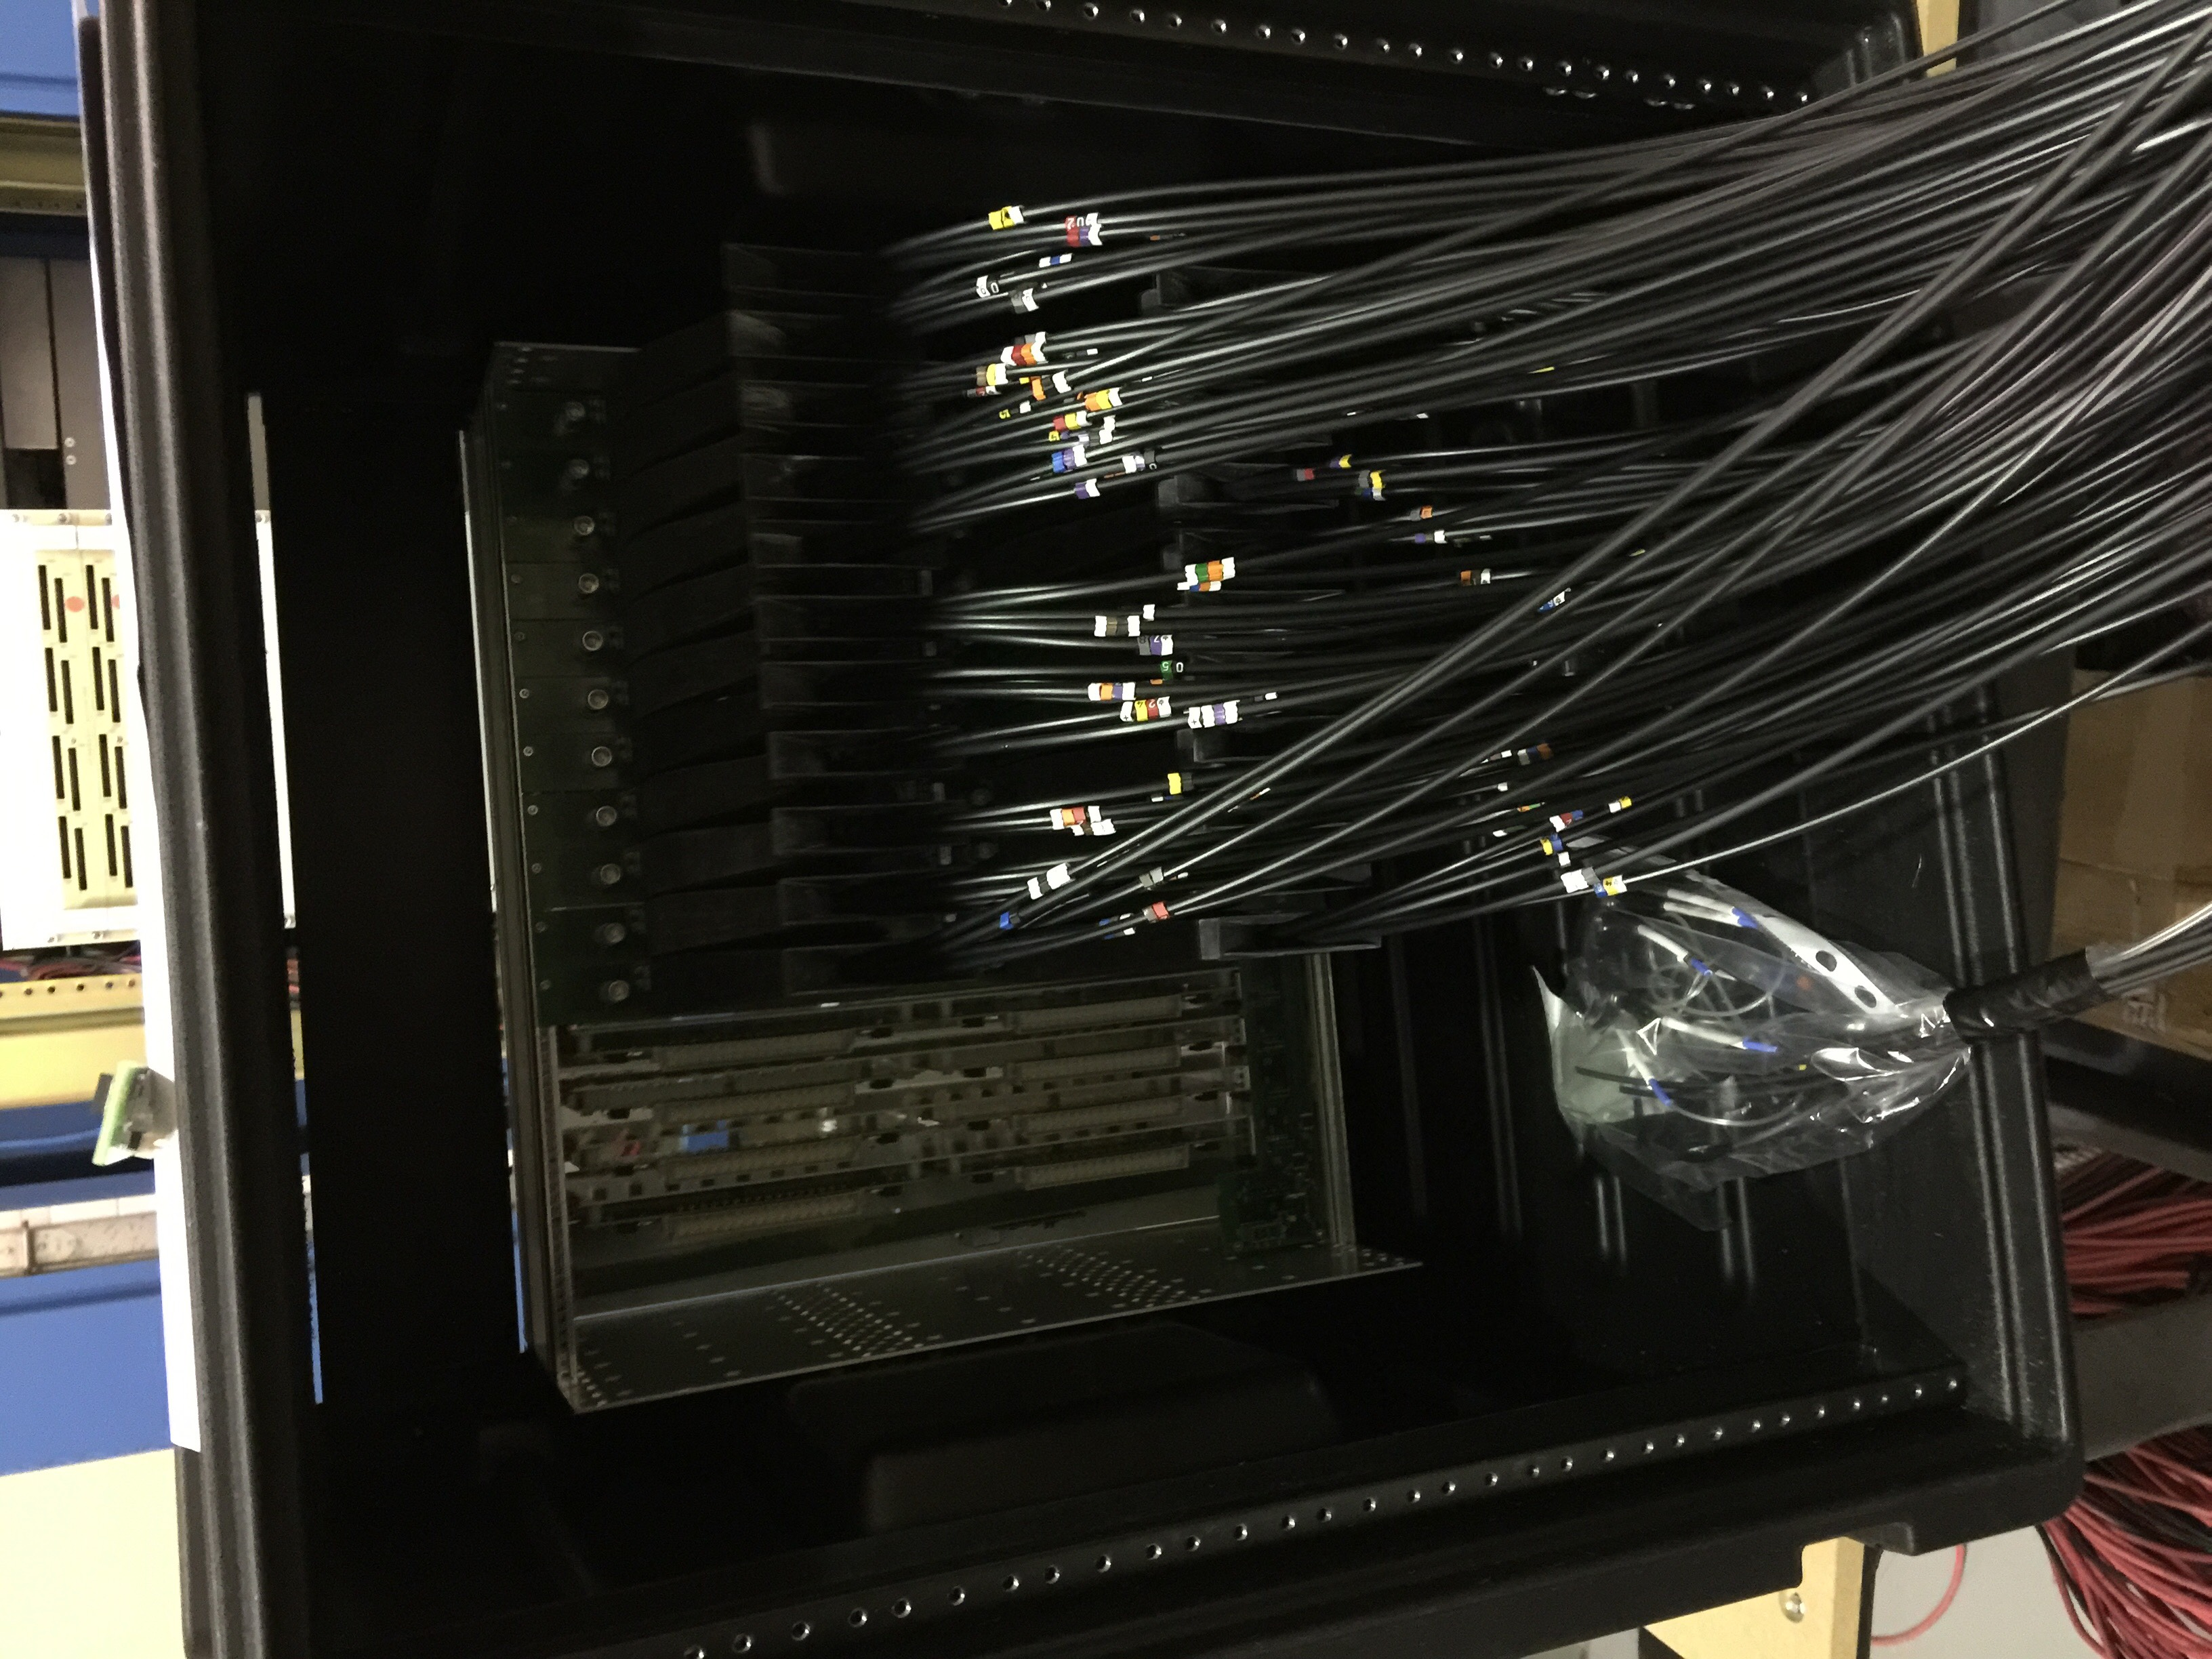
\includegraphics[width=0.7\textwidth]{ImgChap1/JLABTestingCrate}
	\caption{Setting up the hodoscope for testing at Jefferson Lab.}		
	\label{JLABCrate}
\end{figure}

\begin{figure}
	\centering
	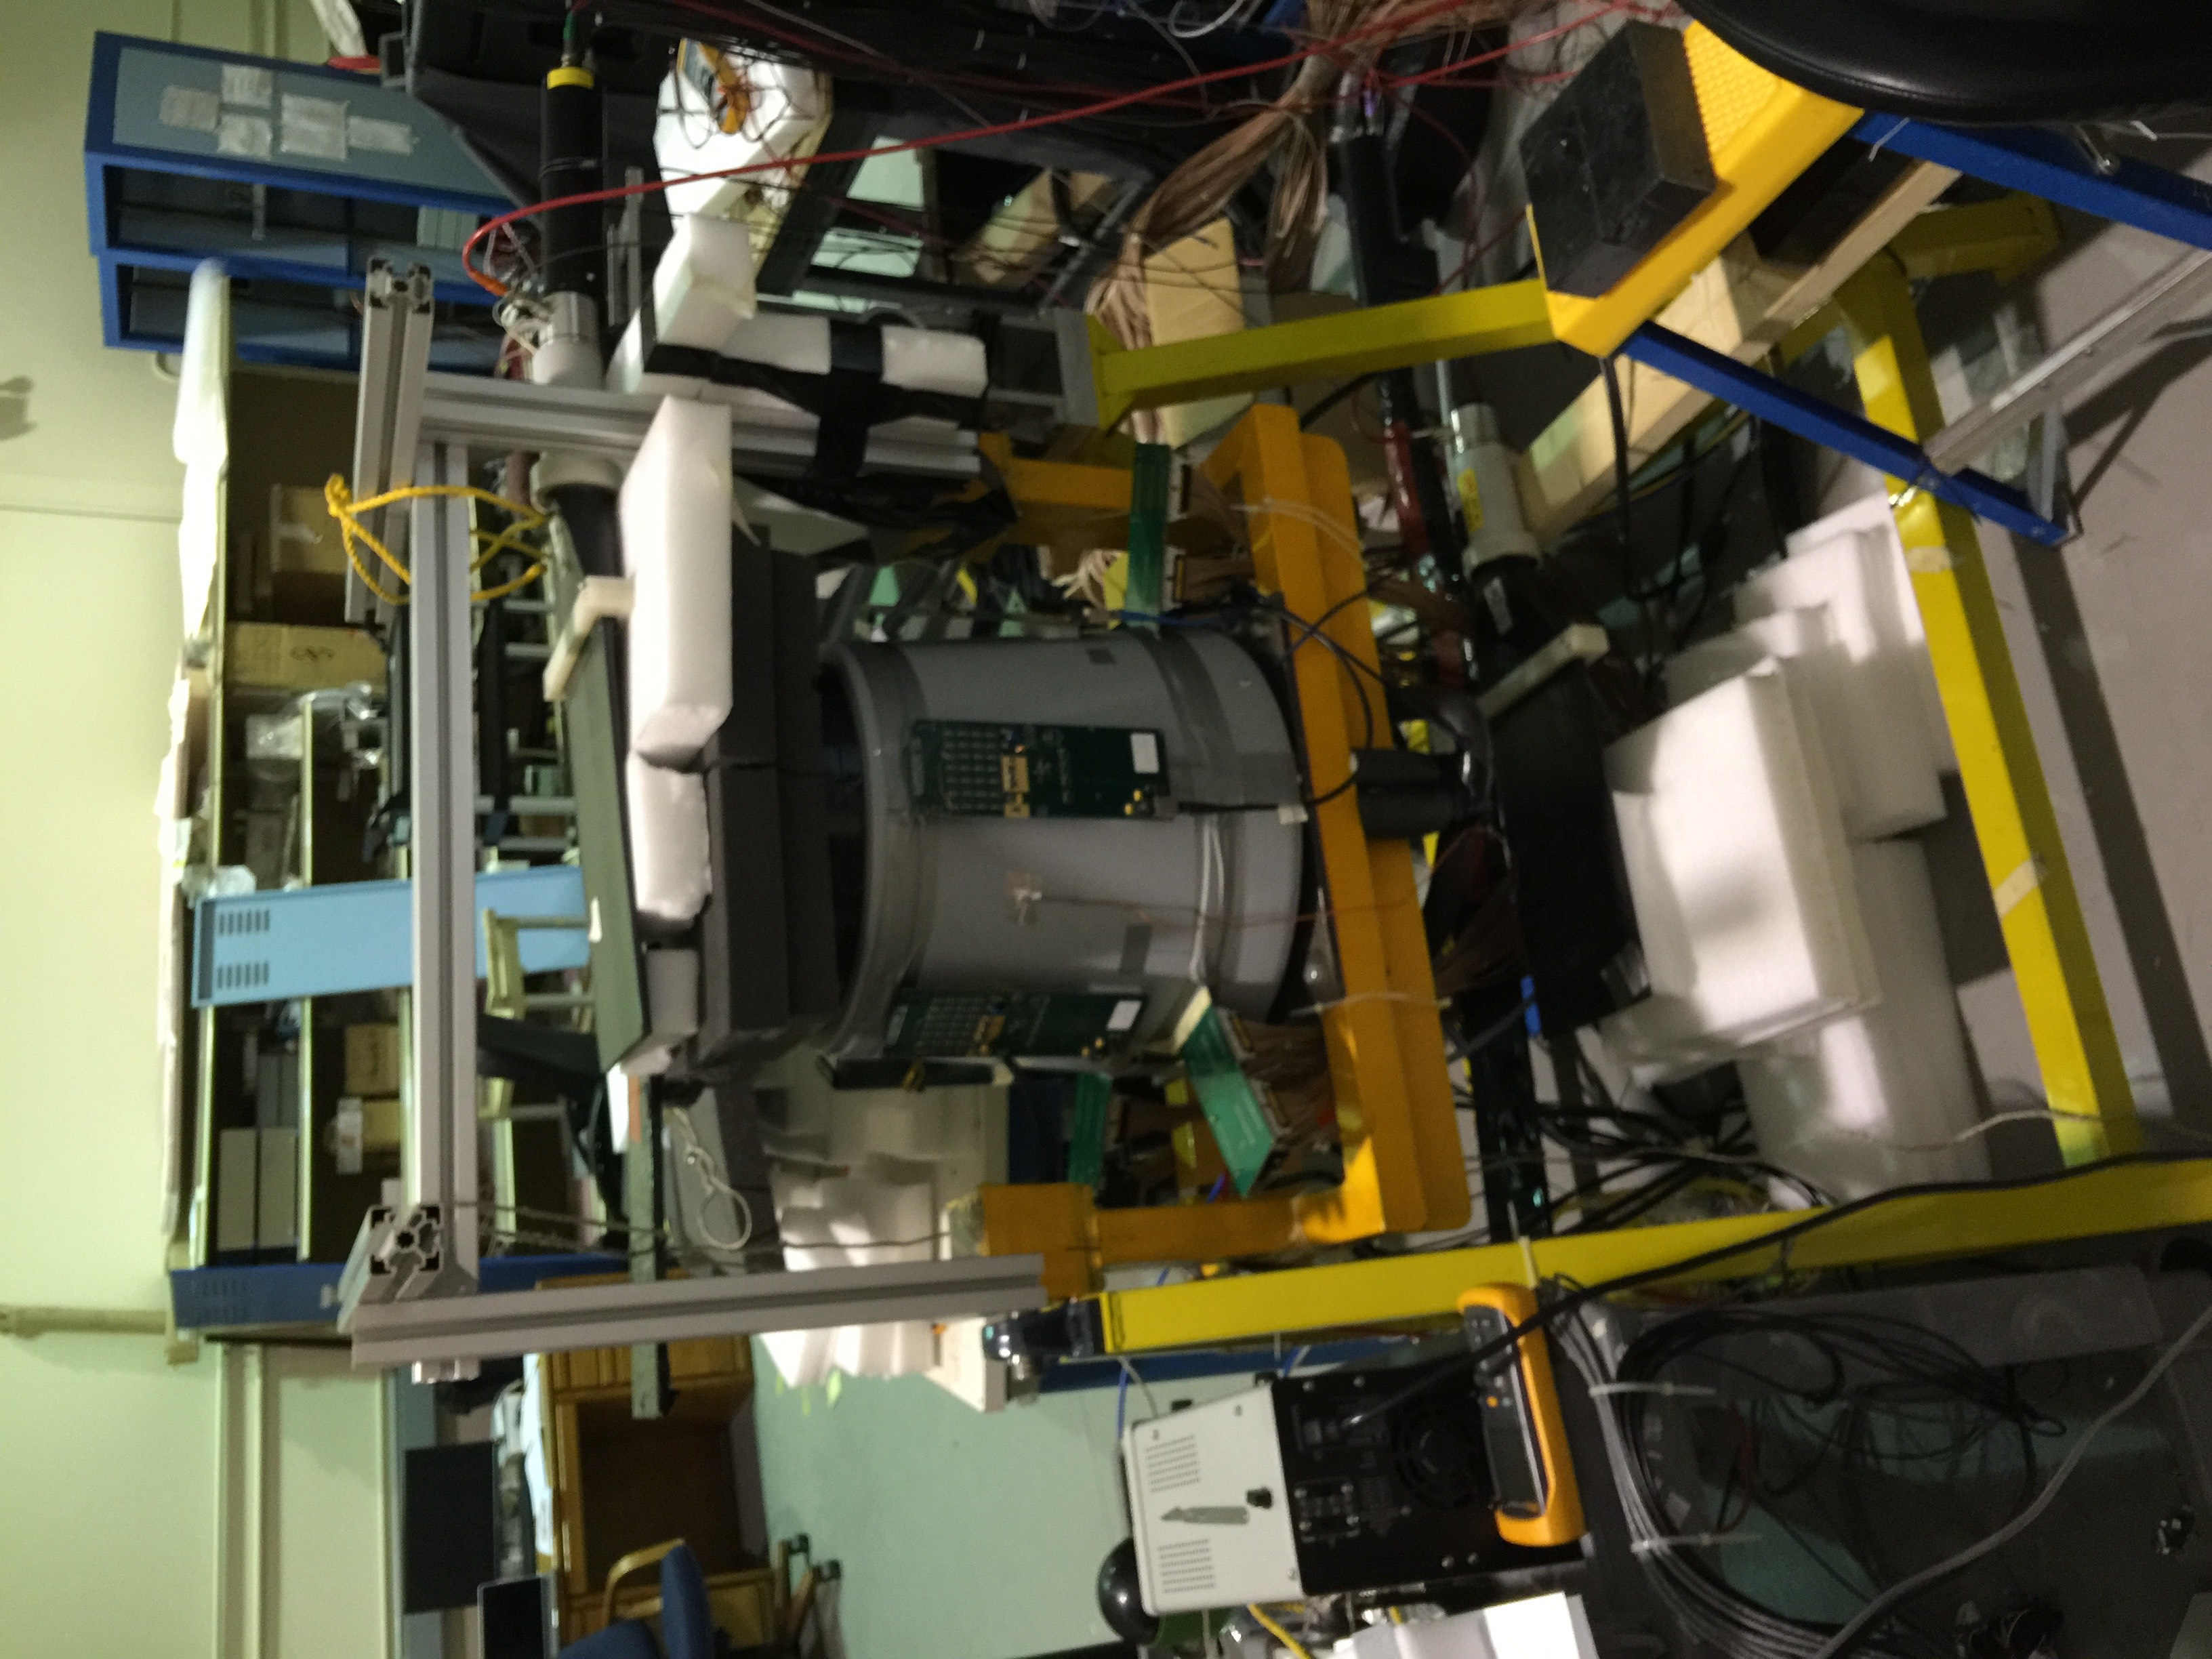
\includegraphics[width=0.7\textwidth]{ImgChap1/JLABTestingHodo}
	\caption{Setting up the hodoscope for testing at Jefferson Lab.}		
	\label{JLABHodo}
\end{figure}

\begin{figure}
	\centering
	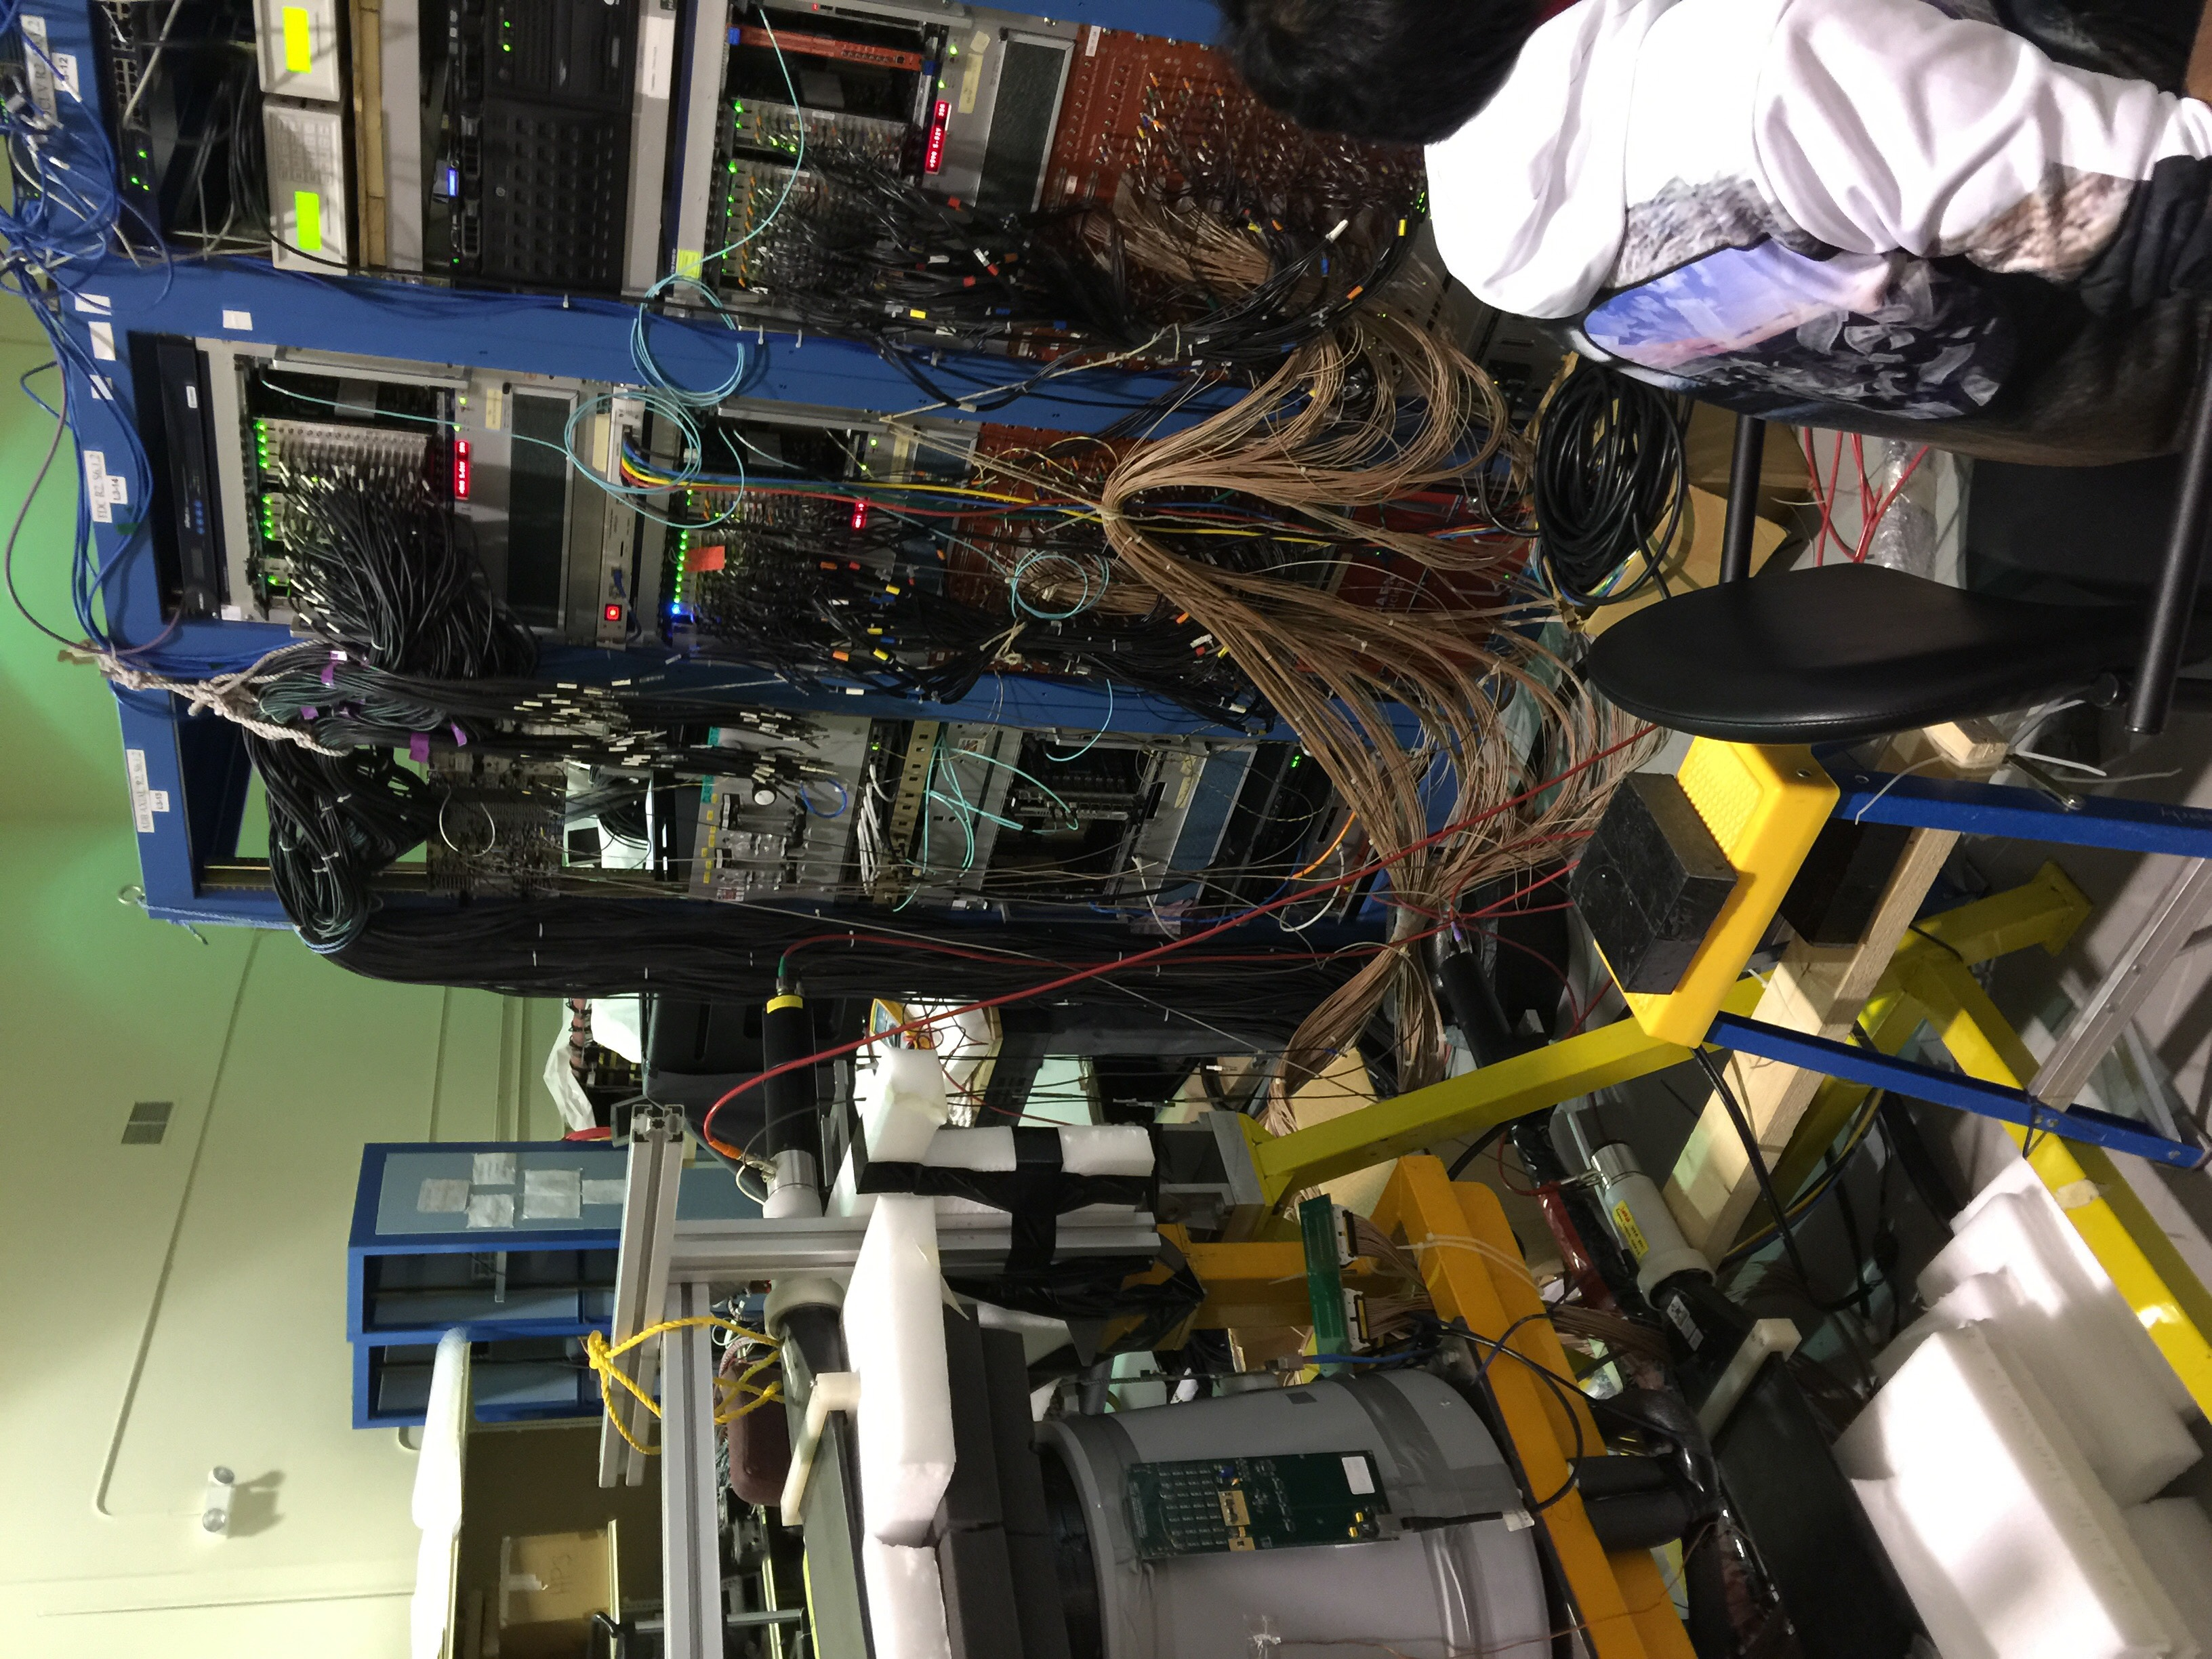
\includegraphics[width=0.7\textwidth]{ImgChap1/JLABTestingElectronics}
	\caption{Setting up the hodoscope for testing at Jefferson Lab.}		
	\label{JLABElec}
\end{figure}


\section{Detector Longevity}
Expected effect of running on the detector.

Radiation damage.

Electronic issues.
			
\section{Software Development}
			
Stuff on the operational controls mainly developed by Nick and Gary and how it will be used to operate and calibrate the detector system.
			
Something on the slow controls.
			
How will the trigger system work for the detector while in operation.
			
\section{Commissioning}
Calibrating, optimising, fixing any problems and resolving any unforeseen issues.

\section{Future development}
Upgrades to the electronics crate to provide fan cooling to the SiPM boards. Actually now completed! Allowing them to be running at a higher operating voltage.